\documentclass[11pt]{article}

% fullpage is a little ambiguous -- two different ones around....
% \usepackage{fullpage}
% set margins ourselves
\typeout{Style Option FULLPAGE Version 2 as of 15 Dec 1988}
\topmargin 0pt
\advance \topmargin by -\headheight
\advance \topmargin by -\headsep
\textheight 8.9in
\oddsidemargin 0pt
\evensidemargin \oddsidemargin
\marginparwidth 0.5in
\textwidth 6.5in

\usepackage{graphicx}
\usepackage{palatino}
\usepackage[scaled=0.92]{helvet}
\usepackage[scaled=0.985]{couriers}

\usepackage{url}
\usepackage{cite}
\usepackage{multicol}
\usepackage{listings}
\usepackage{color}
\usepackage{subfigure}
\usepackage{ifpdf}
\usepackage{epsfig}

\ExecuteOptions{letter}

\newcommand{\Cpp}{C\kern-0.05em\texttt{+\kern-0.03em+}}
\newcommand{\conceptCpp}{Concept\Cpp}
\newcommand{\concept}[1]{\textsf{#1}}
\newcommand{\halfline}{\vspace{-1.5ex}}

\newenvironment{commentenv}[1]{\begin{list}{}{}\item[]{\sc [#1:}
}{{\rm {\sc End of comment.]}} \end{list}}

%\long\gdef\comment#1#2{[\textsc{#1}: \textsf{#2}]}
\long\gdef\comment#1#2{}
\long\gdef\anju#1{\comment{Anju}{#1}}
\long\gdef\todo#1{\comment{To do}{#1}}

\newcommand{\code}[1]{\lstinline[basicstyle=\sffamily]{#1}}
\newcommand{\func}[1]{\lstinline[basicstyle=\sffamily]{#1()}}
\newcommand{\keyword}[1]{\emph{#1}}
\newcommand{\ConceptCpp}{ConceptC\kern-0.05em\texttt{+\kern-0.03em+}}
\newcommand{\MPIpp}{MPI\kern-0.05em\texttt{+\kern-0.03em+}}
\newcommand{\Cilkpp}{Cilk\kern-0.05em\texttt{+\kern-0.03em+}}
\newcommand{\Charmpp}{Charm\kern-0.05em\texttt{+\kern-0.03em+}}
\newcommand{\tablefont}{\fontsize{9}{15}\selectfont}
\renewcommand{\emph}{\textit}

\lstdefinestyle{basic}{showstringspaces=false,columns=fullflexible,language=C++,escapechar=@,xleftmargin=1pc,%
basicstyle=\small\sffamily,
commentstyle=\mdseries,
moredelim=**[is][\color{white}]{~}{~},
morekeywords={concept,model,requires,where,reduction},
literate={->}{{$\rightarrow\;$}}1 {<-}{{$\leftarrow\;$}}1 {=>}{{$\Rightarrow\;$}}1,
}

\makeatletter

\renewenvironment{thebibliography}[1]
     {\section*{\refname
        \@mkboth{\MakeUppercase\refname}{\MakeUppercase\refname}}%
      \list{\@biblabel{\@arabic\c@enumiv}}%
           {\settowidth\labelwidth{\@biblabel{#1}}%
            \leftmargin\labelwidth
            \advance\leftmargin\labelsep
            \@openbib@code
            \usecounter{enumiv}%
            \let\p@enumiv\@empty
            \renewcommand\theenumiv{\@arabic\c@enumiv}}%
      \sloppy\clubpenalty4000\widowpenalty4000%
      \sfcode`\.\@m}
     {\def\@noitemerr
       {\@latex@warning{Empty `thebibliography' environment}}%
      \endlist}

\def\Box{{\ \vbox{\hrule\hbox{%                                            
   \vrule height1.3ex\hskip0.8ex\vrule}\hrule
  }}\par}

%%%%%%%%%%%%%%%%%%%%%%%%%%%%%%%%%%%%%%%%%%%%%%%%%%%%%%%
% A subfigure environment that can hold verbatim text %
%%%%%%%%%%%%%%%%%%%%%%%%%%%%%%%%%%%%%%%%%%%%%%%%%%%%%%%

\newbox\subfigbox % Create a box to hold the subfigure. 
\makeatletter 
\newenvironment{subfloat}% % Create the new environment. 
{\def\caption##1{\gdef\subcapsave{\relax##1}}% 
\let\subcapsave=\@empty % Save the subcaption text. 
\let\sf@oldlabel=\label 
\def\label##1{\xdef\sublabsave{\noexpand\label{##1}}}% 
\let\sublabsave\relax % Save the label key. 
\setbox\subfigbox\hbox 
\bgroup}% % Open the box... 
{\egroup % ... close the box and call \subfigure. 
\let\label=\sf@oldlabel 
\subfigure[\subcapsave]{\box\subfigbox}}% 
\makeatother 
 

\lstset{language=C++,style=basic}

\title{PFunc: An Overview}

\author{Prabhanjan Kambadur}

\begin{document}

\maketitle

\tableofcontents

\pagebreak

\section{Introduction}
\label{sec:introduction}

% General introduction
This tutorial helps you learn to use PFunc, short for Parallel Functions, a
lightweight and portable library that provides C and \Cpp{} APIs to express
task parallelism. 
%
PFunc enables programmers to focus on developing parallel algorithms and
specify low-level and high-level tasks to parallelize instead of working with
native threading libraries such as POSIX and Windows threads.
%
Although there are several task libraries, PFunc is unique in that its features
are a strict superset of the features offered by current solutions for task
parallelism.  
%
Specifically, PFunc extends the feature set of current solutions with custom
task scheduling, task priorities and task affinities.
%
In addition, PFunc offers task groups for SPMD-style programming and multiple
task completion notifications for parallel execution of DAGs. 
%
PFunc's extended feature set is geared towards helping knowledgeable users
optimize their application performance. 
%

\subsection{Organization}
\label{subsec:organization}
%
\begin{figure}[t]
\centering
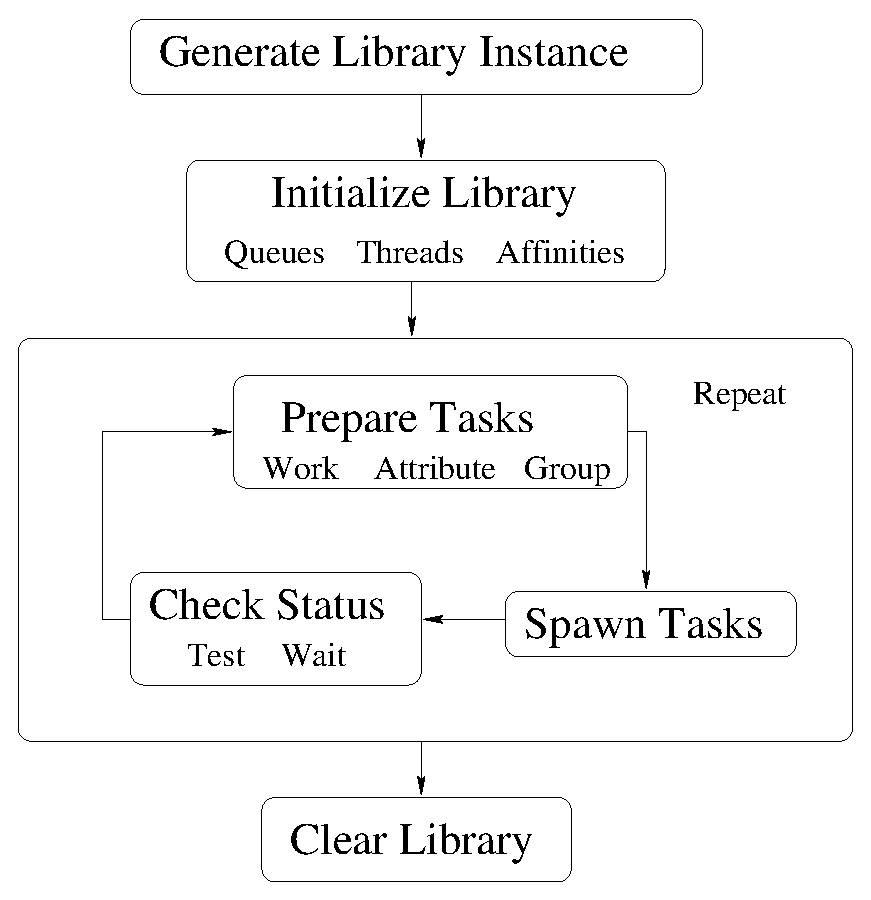
\includegraphics[width=0.5\textwidth]{figs/life-cycle}
\caption{Life-cycle of a PFunc application.}
\label{fig:life_cycle}
\end{figure}
%
Figure~\ref{fig:life_cycle} depicts the life-cycle of a PFunc
application. 
%
First, the library is initialized. Then, tasks are repeatedly spawned and
executed in parallel.  Finally, the library instance is cleared.
%
This tutorial is organized to reflect the life-cycle of PFunc applications.
%
The table below gives a brief summary of each section.
% 
\begin{center}
\begin{tabular}{|c|l|}
\hline
Section & Explanation \\
\hline
Section~\ref{sec:introduction} & Introduction to the tutorial.\\
\hline
Section~\ref{sec:install} & Installation and package information.\\
\hline
Section~\ref{sec:generate} & Generating PFunc's library instance description.\\
\hline
Section~\ref{sec:initialize} & Initializing the library.\\
\hline
Section~\ref{sec:spawn} & Creating, spawing, and waiting for tasks.\\
\hline
Section~\ref{sec:fibonacci} & A complete Fibonacci example in C. \\
\hline
Section~\ref{sec:pack} & Packing and unpacking arguments in C. \\
\hline
Section~\ref{sec:attribute} & Setting task attributes. \\
\hline
Section~\ref{sec:group} & Group operations in PFunc.\\
\hline
Section~\ref{sec:sync} & Locks and atomic operations.\\
\hline
Section~\ref{sec:loops} & Higher-level parallel loop primitives.\\
\hline
Section~\ref{sec:exception} & Handling exceptions.\\
\hline
Section~\ref{sec:perf} & Gather hardware statistics using PFunc and PAPI.\\
\hline
Section~\ref{sec:design} & A detailed description of PFunc's design.\\
\hline
Section~\ref{sec:custom} & Customizing PFunc. \\
\hline
\end{tabular}
\end{center}


\pagebreak

\section{Installation}
\label{sec:install}
%
This document contains basic information required to install and start using
PFunc. 
%
Please take the time to read through it as there might be subtleties in the
build process that might influence behavior of PFunc, and ultimately, your
application. 
%

\subsection{Software Requirements}
\label{subsec:install_requirements}
PFunc uses CMake to configure and build itself. We selected CMake for its
portability across Windows, Linux and Unix platforms. 
%
So, in order to configure and build PFunc, it is required that CMake be
installed on your system.
%
To obtain a copy of CMake, please visit \texttt{www.cmake.org}. PFunc requires
CMake version 2.6 or later.
%
To build documentation, PFunc requires these additional software: doxygen,
latex, dvips, ps2pdf, perl, and makeindex; however, these are not required 
if users do not intend to build documentation.

\subsection{Supported Platforms}
\label{subsec:supported_platforms}
%
PFunc is written in standards conformant C++, and as such, it should work with
most C++ compilers. 
%
However, because as PFunc makes heavy use of templates, it is recommended to
get the latest C++ compilers. 
%
Furthermore, as PFunc makes use of low-level assembly code for atomic
operations, it is guaranteed to work \textit{only} on certain architectures.
%
The table below lists all the platforms on which PFunc has been tested.

\begin{center}
\begin{tabular}{|c|c|c|}
\hline
Operating System & Architecture & Compiler \\
\hline
Windows & Visual Studio Express 10.0 & x86\_32 and x86\_64 \\
\hline
Linux, kernel $\ge{}$2.6 & GCC $\ge{}3.4.6$ & x86\_32, x86\_64, ppc32, and ppc64 \\
\hline
AIX $\ge{}5.3$ & GCC $\ge{}3.4.6$ & ppc2 and ppc64 \\
\hline
OS X $\ge{}10.5$ & GCC $\ge{}3.4.6$ & x86\_32 and x86\_64 \\
\hline
\end{tabular}
\end{center}

\subsection{Header Files and \code{libpfunc}}
%
To use PFunc's \Cpp{} interface, it is sufficient to configure PFunc and use 
the header files; on the other hand, to use the C interface, it is necessary 
to link against \code{libpfunc}.
%
The table below lists all the header files and their contents.
%
\begin{center}
\begin{tabular}{|c|c|c|}
\hline
Header & Language & Contents \\
\hline
\code{pfunc/pfunc.h} & C & \textit{All} definitions for task-based parallelization. \\
\hline
\code{pfunc/pfunc.hpp} & \Cpp{} & \textit{All} definitions for task-based parallelization. \\
\hline
\code{pfunc/parallel\_for.hpp} & \Cpp{} & Necessary to use \code{pfunc::parallel\_for}. \\
\hline
\code{pfunc/parallel\_reduce.hpp} & \Cpp{} & Necessary to use \code{pfunc::parallel\_reduce}. \\
\hline
\code{pfunc/parallel\_while.hpp} & \Cpp{} &  Necessary to use \code{pfunc::parallel\_while}. \\
\hline
\code{pfunc/pfunc\_atomics.h} & C,\Cpp{} & Necessary to PFunc atomics. \\
\hline
\code{pfunc/utility.h} & C,\Cpp{} & Necessary to use timers and other utilities. \\
\hline
\end{tabular}
\end{center}

\subsection{Configuration Options}
%
Configuration is necessary to use either the C or the \Cpp{} interfaces. 
%
During this phase, PFunc (using CMake) gathers all platform specific
information to provide the most optimal execution to its users.
%
There are a variety of options available for configuring PFunc; a detailed list
of these options is available using the command \code{cmake -i}.
%
We briefly describe the important options and their default values below.
%
\paragraph{CMAKE\_BUILD\_TYPE}
The available choices are \code{Release}, \code{Debug} and
\code{RelWithDebugInfo}; the default is \code{Release}.

\paragraph{CMAKE\_INSTALL\_PREFIX}
The value of this variable is used as the base installation location for PFunc;
the default value is \code{/usr/local}.

\paragraph{BUILD\_EXAMPLES}
The available choices are \code{ON|On} and \code{OFF|Off}; by default, this 
option is turned \code{ON}. 
%
Enabling this builds the examples that are provided with the distribution.

\paragraph{BUILD\_PERF\_TESTS}
The available choices are \code{ON|On} and \code{OFF|Off}; by default, this 
option is turned \code{OFF}.
%
Enabling this builds the performance tests that are provided with the
distribution.

\paragraph{BUILD\_TUTORIAL}
The available choices are \code{ON|On} and \code{OFF|Off}; by default, this 
option is turned \code{OFF}.
%
Enabling this builds the PFunc tutorial.

\paragraph{BUILD\_DOCS}
The available choices are \code{ON|On} and \code{OFF|Off}; by default, this 
option is turned \code{OFF}.
%
Enabling this option builds in-code documentation. 

\paragraph{USE\_EXCEPTIONS}
This option is used to turn on exception handling (\code{ON|On}) in PFunc; by
default, this option is turned \code{OFF|Off}.

\paragraph{USE\_PAPI}
This option is used to turn on hardware performance profiling (\code{ON|On}) in 
PFunc; by default, this option is turned \code{OFF|Off}.
%
Note that PAPI needs to be installed in order for performance profiling to 
work.

\subsection{Installation}
For a clean installation process, we recommend an out-of-source build; however,
the in-source build works just as well. 
%
Given below are the basic installation instructions for PFunc on Linux/OS
X/AIX:

\begin{list}{\labelitemi}{\leftmargin=0em}
\item
Get a copy of PFunc; for the sake of this installation guide, let us assume
that PFunc's sources have been checked out in the directory
\code{/home/anon/pfunc}.

\item
\code{\#cd /home/anon/ && mkdir pfunc-build}

At the end of this step, we have created \code{/home/anon/pfunc} and 
\code{/home/anon/pfunc-build}.

\item
\code{\#cd /home/anon/pfunc-build}

\item
\code{\#cmake /home/anon/pfunc -DCMAKE\_INSTALL\_PREFIX=/home/anon/pfunc-install}

At this step, we are configuring PFunc and have choosen to install the 
files in \code{/home/anon/pfunc-install}. 
%
Once configuration is done, the following targets are available to be built by
the native build-system: 
  \begin{itemize}
  \item \code{pfunc}, builds the static library \code{libpfunc}
  \item \code{tutorial}, builds the tutorial if BUILD\_TUTORIAL was ON.
  \item \code{doc}, build documentation if BUILD\_DOCS was ON.
  \item \code{all},  builds all the selected targets.
  \item \code{clean}, removes all the object files.
  \item \code{install}, installs the targets to the selected prefix.
  \item \code{uninstall}, does the obvious.
  \item \code{examples}, builds examples if BUILD\_EXAMPLES was ON.
  \item \code{perf\_tests}, builds performance tests if BUILD\_PERF\_TESTS was ON.
  \end{itemize}
\end{list}

%
\subsection{Caveat}
PFunc is written completely in \Cpp{}; that is, \code{libpfunc} is a \Cpp{}
library that provides C-bindings. 
%
To build a C executable using \code{libpfunc}, you \textit{may}  
need to link against the \Cpp{} standard library (\code{libstdc++} on most 
machines and \code{libC} on AIX).
%
When building the C examples and performance tests, PFunc's configuration
mechanism checks for the presence of these libraries. 
%
Unfortunately, due to a shortcoming in CMake, the library has to be named
\code{libstdc++.[so|a]} or \code{libC.[so|a]}. 
%
Usually, what you find on your system will be \code{libstdc++.so.[0-9]}, with a
symbolic link to \code{libstdc++.so}. 
%
In the oft-chance that this symbolic link is missing, the C
examples will fail to build. 
%
In this case, manually create a symbolic link to \code{libstdc++} to fix this 
issue.


\pagebreak

\section{Choosing The Right PFunc}
\label{sec:generate}
%
\begin{table}
\begin{center}
\begin{tabular}{|c|c|}
\hline
Feature & Default \\
\hline
\code{Scheduling policy} & \code{cilkS} \\
\hline
\code{Compare} & \func{std::less<int>} \\
\hline 
\code{Function object} & \code{struct \{ virtual void operator()() = 0; \};} \\
\hline
\end{tabular}
\end{center}
\caption{Default values for PFunc's template parameters.}
\label{tbl:default}
\end{table}
%
PFunc is a templated library; the first step is, therefore, to generate the 
concrete type that will be used as the library instance (\Cpp{} only).
%
PFunc takes three template parameters: \code{scheduling policy},
\code{compare}, and \code{function object}.
%
For most users, it is sufficient to provide default values to the template 
parameters that are used in PFunc; Table~\ref{tbl:default} lists the default
values for each of the three template parameters.
%
We briefly describe the roles of each of these template parameters; for a more
detailed description, please see Sections~\ref{sec:design} and~\ref{sec:custom}.
%
\begin{list}{\labelitemi}{\leftmargin=0em}
% Scheduling policy
\item \code{Scheduling policy:}
This template parameter names the scheduling policy to be used; the built-in
values that can be used are \code{cilkS}, \code{lifoS}, \code{fifoS}, and
\code{prioS}.

% Compare
\item \code{Compare:}
This template parameter represents the ordering operator for task priorities; 
for the built-in scheduling policies, it is used only for \code{prioS}.

% Functor
\item \code{Function object:}
This template parameter determines the type of the function objects that are 
parallelized; when default value is choosen for this parameter, all function 
objects the need to be parallelized are required to inherit from a abstract
base class.
\end{list}
%
The code below summarizes how a library instance description can be 
generated.
%
\begin{center}
\begin{minipage}{0.75\textwidth}
\begin{lstlisting}
typedef pfunc::generator<cilkS, /* scheduling policy */
                         pfunc::use_default, /* compare */
                         pfunc::use_default> my_pfunc; /*function object*/
\end{lstlisting}
\end{minipage}
\end{center}
%
Here, we have generated an new library instance description of PFunc by
choosing the Cilk-style scheduling policy. 
%
The values for the \code{compare} and \code{function object} features are
allowed to be defaults; In fact, It is possible to use
\code{pfunc::use_default} for all the features (Figure~\ref{tbl:default}).  
%
PFunc automatically chooses sensible values for the features in this case.  
%
The type \code{my\_pfunc} thus generated in our example
is a custom instance that can be used to parallelize user applications. 
%
In PFunc, there are four important types that users are exposed to:
\code{attribute}, \code{group}, \code{task} and \code{taskmgr}.  
%
Once the required library instance description has been generated, these types
can be accessed as follows:

\begin{center}
\begin{minipage}{0.4\textwidth}
\begin{lstlisting}
typedef my_pfunc::attribute attribute; 
typedef my_pfunc::group group; 
typedef my_pfunc::task task; 
typedef my_pfunc::taskmgr taskmgr; 
\end{lstlisting}
\end{minipage}
\end{center}

% attribute
Objects of type \code{attribute} allow users to control the execution of
spawned tasks by setting attributes such as task priority and task affinity
(see Section~\ref{sec:attribute}).
% group
Objects of type \code{group} can be used to create collaborations of tasks that
can communicate with each other using point-to-point message passing and
barrier synchronization (see Section~\ref{sec:group}).
% task
Objects of type \code{task} are used as references to spawned tasks, which 
can be passed to other tasks. The ability to pass task references is crucial
for the support of multiple task completion notifications (see
Section~\ref{sec:spawn}).
% taskmgr
Finally, objects of type \code{taskmgr} manage threads and their task
queues, and are responsible for task scheduling (see Section~\ref{sec:spawn}).

\subsection{C}
In C, both because of the lack of support for generic programming and the
pitfalls of over-using preprocessor macros, PFunc pre-generates the library
instance descriptions for the users; the definitions for these are present in
\code{pfunc/pfunc.h}.
%
The users are merely required to then select the right set of functions from
the available sets of pre-generated functions; each set is denoted by a 
common prefix and is given in the table below:
%
\begin{center}
\begin{tabular}{|c|c|c|c|}
\hline
Instance description & Scheduling policy & Compare, priority & Function type \\
\hline
\code{pfunc_cilk_*} & Cilk-style & \code{unused} & \code{void (*)(void*)} \\
\hline
\code{pfunc_lifo_*} & Queue & \code{unused} & \code{void (*)(void*)} \\
\hline
\code{pfunc_fifo_*} & Stack & \code{unused} & \code{void (*)(void*)} \\
\hline
\code{pfunc_prio_*} & Priority-based & \code{<} op, \code{int} & \code{void (*)(void*)} \\
\hline
\end{tabular}
\end{center}
%
Like in \Cpp{}, there are four important types exposed to the users:
\code{attribute}, \code{group}, \code{task} and \code{taskmgr}.
%
For example, for the Cilk-style library instance description, the names by
which these types can be accessed are \code{pfunc_cilk_attr_t},
\code{pfunc_cilk_group_t}, \code{pfunc_cilk_task_t} and
\code{pfunc_cilk_taskmgr_t}. 

\paragraph{Caveat} 
As PFunc is implemented completely in \Cpp{}, the C types (\code{attribute,
group, task, taskmgr}) are mere typed pointers to their \Cpp{} counterparts. 
%
Consequently, these types (eg., \code{pfunc_cilk_attr_t},
\code{pfunc_cilk_group_t}, \code{pfunc_cilk_task_t} and
\code{pfunc_cilk_taskmgr_t}) need to be initialized and cleared explicility
using calls to their respective \func{init} and \func{clear} functions. 
%
This notion of initializing and clearing PFunc's C types will be reinforced
throughout the C examples described in this tutorial.


\pagebreak

\section{Initializing PFunc}
\label{sec:initialize}

\begin{figure}
\begin{tabular}{|c|c|l|}
\hline
Parameter & Type & Explanation \\
\hline
Num queues & \code{unsigned int} & Number of task queues to be used. \\
           &                     & Queues are numbered from 0 to N-1. \\
\hline
Num threads per queue & \code{unsigned int[]} & Number of threads to work on each queue. \\
                      &                       & Allows a $m\times{}n$ mapping. \\
                      &                       & $1\times{}n$ mapping represents work-sharing (thread-pools). \\
                      &                       & $n\times{}1$ mapping represents work-stealing (Cilk-style). \\
\hline
Thread affinities & \code{unsigned int[][]} & Affinity of each thread in each queue to a processor. \\
                  &                         & Processors are numbered from 0 to N-1. \\
                  &                         & Default values are accepted. \\
\hline
\end{tabular}
\caption{Table depicting the three parameters that are needed to initialize 
PFunc's runtime.}
\label{fig:init}
\end{figure}

% Mention that there are two ways of doing things.
Once the appropriate library instance description has been generated, the next
step is to initialize the PFunc runtime. 
%
PFunc's runtime is encapsulated by objects of type \code{taskmgr}; each object
of type \code{taskmgr} encapsulates a task scheduling policy, a number of task
queues into which tasks can be placed, and threads that are attached to these
task queues, which execute the tasks.
%
In fact, the words ``runtime'' and \code{taskmgr} can be used interchangably.
%
Typically, there is one object of type \code{taskmgr} per application run; 
however, 
users can create as many object instances of type \code{taskmgr} as
they deem necessary.
%
For example, if there are two disjoint sets of
tasks that need to be run simultaneously with different scheduling policies, it
is advisable to create two objects of type \code{taskmgr}. 
%
Each such object of
type \code{taskmgr} represents a separate initialized instance of PFunc's
runtime.
%
PFunc further facilitates users who require just one runtime (\code{taskmgr})
per application run by allowing specification of a global object of type
\code{taskmgr} that can be used as an implicit argument in many function calls.
%
To initialize PFunc's runtime, users are required to provide three pieces of
information: number of queues, number of threads per queue and the affinities
of threads to processors (see Figure~\ref{fig:init}).
%
By tweaking these parameters, users are able to choose from a wide variety of
mappings ranging from centralized work-sharing model to the distributed
work-stealing model. 
%
For example, consider the following code that creates an instance of Cilk-style
runtime with four threads and one queue per thread.
%
\begin{lstlisting}
/* Library instance description */
typedef pfunc::generator<cilkS, pfunc::use_default, parallel_foo> my_pfunc;
@\halfline@
int main () {
  unsigned int num_queues = 4;
  const unsigned int num_threads_per_queue[] = {1,1,1,1};
  const unsigned int affinities[4][1] = {{0},{1},{2},{3}};
  @\halfline@
  /* Create a variable of the type taskmgr */
  my_pfunc::taskmgr my_taskmgr (num_queues, num_threads_per_queue, affinities);
  ...
  return 0; /* PFunc runtime is destroyed when my_taskmgr goes out of scope */
}
\end{lstlisting}

\paragraph{Scheduling Model} In the above example, we choose to have 4 task
queues and 1 thread per queue; that is, thread has its own queue. 
%
Since we choose \code{cilkS} scheduling policy, when a thread runs out of work
on its own queue, it ``steals'' work from other task queues; in fact, all four
built-in scheduling policies (\code{cilkS}, \code{prioS}, {lifoS}, and
\code{fifoS}) follow this stealing model.
%
Hence, this model is called the work-stealing model. 
%
At the other end of the spectrum, if had chosen to have a single queue and put
all our threads on it, it would constitute a work-sharing model. 
%
PFunc also allows users to define an $m\times{}n$ model, which would be a
hybrid between the work-stealing and work-sharing models.  
%
The work-stealing model has been proven to be efficient for running
applications that are written in a divide and conquer model. 
%
In such applications, each thread generates ample tasks to keep itself busy and
avoids the contention associated with having a single task queue. 
%
The best scheduling policy for an application is usually found out by
experimenting with different configurations. 
%
With PFunc, this is as simple as just changing the library instance description
and the initialization of the runtime.

\paragraph{Processor Affinities} 
%
In our example, we also specify the processor affinities for each of the
threads; we bound thread 0 to processor 0, thread 1 to processor 1, thread 2 to
processor 2 and thread 3 to processor 3.
%
Processor affinities are currently only supported on Linux platforms. 
%
By default, each thread can be scheduled to run on \textit{any} of the
available processors (cores). 
%
Binding a thread to a particular processor (core) might results in better cache
resuse for applications running on dedicated machines. 
%
However, setting a thread's affinity also prevents it from being scheduled on
other processors (cores). 

\paragraph{How many threads?} 
%
The total number of threads that are created can be calculated by multiplying
the number of queues with the number of threads in each queue. 
%
In our example, we are creating 4 threads in all; these threads are
created in addition to the main user thread that is already running. 
%
As a general rule, it is recommended to have only as many threads running an
application as there are processors (cores). 
%
For example, on a dual core machine, we recommend creating only two threads,
regardless of the configuration that the users set the threads up in (for
example, $2\times{}1$ or $1\times{}2$). 
%
Creating more threads than processors might result in performance degradation
as threads contend for shared computing resources. 
%
Furthermore, each PFunc runtime initialization (i.e., each object of type
\code{taskmgr}) creates its own threads separate from other instances. 
%
So, exercise caution while having more than one library instance running.

\paragraph{What do the threads do?} As soon as PFunc's runtime is initialized,
the task queues and their corresponding threads are created. 
%
Each thread continually checks on the tasks queues (starting with its own) for
tasks to be executed.
%
However, as such continuous checking for tasks to run can deplete compute
resource, PFunc threads check for tasks a pre-specified number of times
($2\times10^{6}$ by default) before ``yielding'' the processor that they are
running on. 
%
Such yielding behavior allows PFunc applications to co-exist with other
applications without completely holding up compute resources. 
%
However, when the number of threads is $\le{}$ to the number of processors
available to run, and the application is being run on a dedicated machine,
users can opt to never yield threads by increasing the number of attempts made
by each thread before yielding. 
%
The higher the number of attempts made by a thread, the quicker the response
time of a task in the task queue of being picked up by the thread and executed. 
%
The code below demonstrates how the maximum attempts can be changed if it is
not to the user's liking. 
%
\begin{lstlisting}
unsigned int num_attempts;
pfunc::taskmgr_max_attempts_get (my_taskmgr, num_attempts);
if (10000 > num_attempts) pfunc::taskmgr_max_attempts_set (my_taskmgr, 10000);
\end{lstlisting}

\subsection{Initializing in C}
\label{sec:c:init}
%
We now demonstrate how to initialize PFunc when using the C interface. 
%
For ease of understanding, we initialize to the same specification as the
\Cpp{} example above.
%
\begin{lstlisting}
int main () {
  unsigned int num_queues = 4;
  const unsigned int num_threads_per_queue[] = {1,1,1,1};
  const unsigned int affinities[4][1] = {{0},{1},{2},{3}};
  pfunc_cilk_taskmgr_t cilk_tmanager;
  @\halfline@
  /* Initialize a global instance of the library */
  pfunc_cilk_taskmgr_init (&cilk_tmanager, num_queues, num_threads_per_queue, affinities);
  ...
  /* Clear the global instance of the library */
  pfunc_cilk_taskmgr_clear (&cilk_tmanager);
  @\halfline@
  return 0;
}
\end{lstlisting}
%
Immediately, two differences can be seen from the \Cpp{} example. 
%
First, as we are programming in C, PFunc is initialized using a function call
(\func{pfunc_cilk_taskmgr_init} in this case) rather than by constructors.
%
Second, unlike in \Cpp{}, PFunc's runtime needs to be explicitly cleared to
release all the resources allocated by PFunc (using
\func{pfunc_cilk_taskmgr_clear} in this case).

\subsection{Using global runtimes}
%
In most cases, only one object of type \code{taskmgr} (one runtime) is
required. 
%
Under such circumstances, it becomes tedious to explicitly specify the correct
runtime to use when spawning tasks. 
%
To avoid this, PFunc allows users to set up a global runtime and use it as the
default runtime when a specific runtime (object of type \code{taskmgr}) is not
specified in the various PFunc function calls. 
%
In following \Cpp{} code sample, we set up a global runtime and then proceed to
change the number of attempts made by each thread to check for the availability
of a task before yielding control to the thread scheduler.

\begin{lstlisting}
typedef pfunc::generator<cilkS, pfunc::use_default, parallel_foo> my_pfunc;
@\halfline@
int main () {
  unsigned int num_queues = 4;
  const unsigned int num_threads_per_queue[] = {1,1,1,1};
  const unsigned int affinities[4][1] = {{0},{1},{2},{3}};
  unsigned int num_attempts;
@\halfline@
  /* Create a variable of the type taskmgr */
  my_pfunc::taskmgr my_taskmgr (num_queues, num_threads_per_queue, affinities);
@\halfline@
  /* Set up my_taskmgr as the global runtime */
  pfunc::init (my_taskmgr);
@\halfline@
  /* Change the number of attempts if necessary */
  pfunc::taskmgr_max_attempts_get (num_attempts);
  if (10000 > num_attempts) pfunc::taskmgr_max_attempts_set (10000);
@\halfline@
  /* Clear my_taskmgr as the global runtime */
  pfunc::clear ();
@\halfline@
  return 0; /* my_taskmgr is destroyed when my_taskmgr goes out of scope */
}
\end{lstlisting}
%
The global run time is set up by first initializing an object of the type
\code{taskmgr} (\code{my_taskmgr}) as before and then using the function
\func{init} to specify the use of \code{my_taskmgr} as the global runtime. 
%
Corresponding to this, it is necessary to clear the global runtime using the
function \func{clear}. This does not destroy \code{my_taskmgr}, but merely
unsets the use of \code{my_taskmgr} as the global runtime; this is useful when
users want to switch to using a different object of type \code{taskmgr} as the
global runtime. 
%
Finally, we turn our attention to how setting up the global 
runtime simplifies further function calls. 
%
In our case, we have simply omitted the first argument (meant to be
\code{my_taskmgr}) from calls to the functions \func{taskmgr_max_attempts_set}
and \func{taskmgr_max_attempts_get}. 
%
Similarly, once the global runtime has been set up, users can omit the
\code{taskmgr} argument from the function call.

Figure~\ref{fig:c_global} demonstrates the programmatic equivalent of the above
example in C; to set up and clear the global runtime, we have used the
functions \func{pfunc_cilk_init} and \func{pfunc_cilk_clear} respectively. 
%
The one marked difference from the \Cpp{} example is the addition of the
``\code{_gbl}'' suffix to the name of the functions that operate on the global
runtimes. 
%
Such suffixing is necessary because C does not provide function overloading. 
%
For example, in Figure~\ref{fig:c_global}, the local equivalent of the function
\func{pfunc_cilk_taskmgr_max_attempts_set_gbl} would be
\func{pfunc_cilk_taskmgr_max_attempts_set}.

\begin{figure}
\begin{center}
\begin{minipage}{0.85\textwidth}
\begin{lstlisting}[frame=lrtb]
int main () {
  unsigned int num_queues = 4;
  const unsigned int num_threads_per_queue[] = {1,1,1,1};
  const unsigned int affinities[4][1] = {{0},{1},{2},{3}};
  pfunc_cilk_taskmgr_t cilk_tmanager;
  unsigned int num_attempts;
@\halfline@
  /* Initialize a global instance of the library */
  pfunc_cilk_taskmgr_init (&cilk_tmanager, num_queues, num_threads_per_queue, affinities);
@\halfline@
  /* Set up the global runtime */
  pfunc_cilk_init (&cilk_tmanager);
@\halfline@
  /* Change the number of attempts if necessary */
  pfunc_cilk_taskmgr_max_attempts_get_gbl (&num_attempts);
  if (10000 > num_attempts) pfunc_cilk_taskmgr_max_attempts_set_gbl (10000);
@\halfline@
  /* Clear the global runtime */
  pfunc_cilk_clear (&cilk_tmanager);
@\halfline@
  /* Clear the global instance of the library */
  pfunc_cilk_taskmgr_clear (&cilk_tmanager);
@\halfline@
  return 0;
}
\end{lstlisting}
\end{minipage}
\end{center}
\caption{Setting up a PFunc global Cilk-style runtime in C.}
\label{fig:c_global}
\end{figure}


\pagebreak

\section{Spawning tasks}
\label{sec:spawn}

PFunc allows parallel execution of functions.  Let us explore this notion in a
bit more detail.  A normal function call is executed sequentially.
Furthermore, a sequence of function calls are also executed sequentially.
However, it is often the case that there are function calls that can be
executed at the same time without any harmful side effects.  In such cases, one
can make use of PFunc to execute functions in parallel with respect to each
other.  For example consider the problem of calculating the sum of an integer
array.

\begin{lstlisting}
int array_sum (int a[], int n) {
  int sum = 0;
  int i;
  for (i=0; i<n; ++i)  sum += a[i];

  return sum;
} 
\end{lstlisting}

Now, suppose that we are to sum up an array of 100 elements. We could then 
invoke \func{array_sum} as shown below:

\begin{lstlisting}
int main () {
  int a[100];
  return array_sum (a, 100);
}
\end{lstlisting}

Although this serves our purpose, we could speed up the calculation by 
splitting the array into two and using \func{array_sum} on each part:

\begin{lstlisting}
int main () {
  int a[100];
  return array_sum (a, 50) + array_sum (a+50, 50);
}
\end{lstlisting}

Once we have written the problem in this form, we can see that the two 
invocations of \func{array_sum} can actually be executed in parallel. It is
precisely such things that PFunc allows us to do.

\subsection{Creating work}
In the introductory section above, we saw what PFunc allows us to do.
However, the term \textbf{function} is broad, and as such, PFunc can only accept
functions expressed in a particular form. In this section, we exposit on the
functions that PFunc accepts. In brief, PFunc accepts work in two forms: as
function pointers (C and \Cpp{}), and function objects (\Cpp{} only).  In this
section, we explain the functions and function pointers that are accepted by
PFunc.

\begin{figure}
\centering
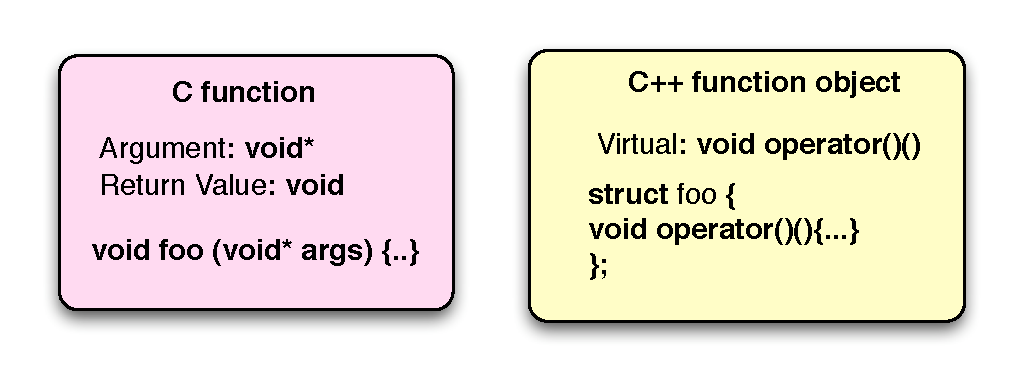
\includegraphics[width=0.6\textwidth]{figs/functors}
\caption{Prototypes of work accepted by PFunc.}
\label{fig:functors}
\end{figure}

\subsubsection{C-style function pointers}
PFunc accepts function pointers of the type \code{void (*)(void*)}. The
example below demonstrates how one such function looks like.

\begin{lstlisting}
void parallel_foo (void* arg) {
  char* string = (char*) arg;
  printf ("PFunc task printing: %s\n", string);
  return;
}
\end{lstlisting}

Note that the function only accepts a single argument of type \code{void*}.
Because of the constraints of a statically typed language, PFunc cannot accept
arbitrary function objects as tasks.  However, PFunc provides two function
calls - \func{pfunc_pack} and \func{pfunc_unpack} to facilitate currying
arguments to parallel functions (see Section~\ref{sec:pack}).

\subsubsection{\Cpp{} function objects}
PFunc also accepts \Cpp{} function objects (overloaded \func{operator()}) as
work. Figure~\ref{fig:functors} depicts the prototype of function objects.
However, using function objects as work requires some attention. As function
objects name concrete types, users must decide if they have more than one
\code{type} of function object that needs to be parallelized. If so, then 
all the function objects must derive from a common base class, which can then
be used as the type of the \code{Function object} feature during library 
instance generation (see Section~\ref{sec:generate}). In the following 
sections, we explain how to generated library instance descriptions for both 
cases.

\begin{list}{\labelitemi}{\leftmargin=1em}
\item \textbf{Single function object:} In this case, for optimal performance, 
it is beneficial to explicitly name the function object that is going to be 
used at library instance description generation time. For example, consider 
the code sample given below:

\begin{lstlisting}
/* Forward declaration */
struct parallel_foo;

/* Library instance description */
typedef pfunc::generator<cilkS, /* scheduling policy */
                         pfunc::use_default, /* compare */
                         parallel_foo> my_pfunc; /*function object*/

struct parallel_foo {
  ...
  void operator()() { ... };
};
\end{lstlisting}

In this case, \code{parallel_foo} is the only function object that can be 
parallelized by the library instance \code{my_pfunc}. As the function object 
is explicitly named, PFunc avoids making virtual function calls when spawning 
tasks. Using one function object to parallelize suffices for many applications
(eg., Fibonacci in Section~\ref{sec:fibonacci}).

\item \textbf{Multiple function objects:} In this case, users are required to
name a common type during library instance description generation and have all
their function objects derive from this type.  To facilitate this case, PFunc
provides a built-in base type that users can derive from. The following example
demonstrates the use of the common base type:

\begin{lstlisting}
/* Library instance description */
typedef pfunc::generator<cilkS, /* scheduling policy */
                         pfunc::use_default, /* compare */
                         pfunc::use_default> my_pfunc; /*function object*/

/* First function object */
struct parallel_foo : public my_pfunc::functor {
  void operator()() { ... };
};

/* Second function object */
struct parallel_bar : public my_pfunc::functor {
  void operator()() { ... };
};
\end{lstlisting}

In the example above, \code{pfunc::use\_default} is used as the value for the
\code{Function object} feature. As a result, PFunc uses a virtual base class
that stipulates \func{operator()}. The type of this class can be accessed from
the generate library instance description using the nested type
\code{::functor}. Now, invocations of \func{operator()} on both
\code{parallel\_foo} and \code{parallel\_bar} can be parallelized.

\end{list}

\subsection{Spawning tasks}
Once we have initialized the library and created work (functions and function
objects), we can parallelize execution of these work packets using PFunc. In 
addition to the work packets, each task is comprised of three additional 
details. These are:

\begin{list}{\labelitemi}{\leftmargin=1em}
\item \code{Attribute:} controls the execution of the task (see
Section~\ref{sec:attribute}).  PFunc provides suitable default value to this
parameter.
\item \code{Group:} enables SPMD-style task groups (see
Section~\ref{sec:group}).  PFunc provides suitable default value to this
parameter.
\item \code{Task handle:} a receipt for the spawned task. This handle can be 
used to query the status of the spawned task.
\end{list}

In \Cpp{}, these types can be accessed as nested types of the generated library
instance description. In C, these types are pre-generated. 

\subsubsection{Spawning tasks in C}
\label{subsubsec:spawn_c}
In this section, we will introduce parallelization of a simple function using 
PFunc by means of an example. Consider the code sample give below.

\begin{lstlisting}
void parallel_foo (void* arg) {
  char* string = (char*) arg;
  printf ("PFunc task number: %s\n", string);
  return;
}

int main () {
  pfunc_cilk_task_t tasks[10];
  unsigned int num_queues = 4;
  const unsigned int num_threads_per_queue[] = {1,1,1,1};
  pfunc_cilk_taskmgr_t cilk_tmanager;
  int i;

  /* Initialize a global instance of the library */
  pfunc_cilk_taskmgr_init (&cilk_tmanager, num_queues, num_threads_per_queue, NULL);

  /* Spawn the tasks */
  for (i=0; i<10; ++i) {
    pfunc_cilk_task_init (&(tasks[i]));
    pfunc_cilk_spawn_c (cilk_tmanager, tasks[i], NULL, NULL, parallel_foo, ltoa(i));
  }

  /* Wait for the tasks and clear the task handle */
  for (i=0; i<10; ++i) {
    pfunc_cilk_wait (cilk_tmanager, tasks[i]);
    pfunc_cilk_task_clear (&(tasks[i]));
  }

  /* Clear the library */
  pfunc_cilk_taskmgr_clear (&cilk_tmanager);

  return 0;
}
\end{lstlisting}

In the above example, we have parallelized execution of \func{parallel_foo}
using PFunc. First, we initialize the Cilk-style library instance using the
function call \func{pfunc_cilk_taskmgr_init}. In this example, we use task
queues, 1 thread per queue and allow default values for thread affinities.
Second, we spawn 10 instances of \func{parallel_foo} using the function
\func{pfunc_cilk_spawn_c}. In this example, we choose to use the default value
(NULL) for both \code{attribute} and \code{group}. Notice that the task handle
has to be initialized (using \func{pfunc_cilk_task_init}) prior to its use in
\func{pfunc_cilk_spawn_c}. This is required as the C types are mere pointers to
their \Cpp{} counterparts. Third, we wait for the spawned tasks to finish using
\func{pfunc_cilk_wait} before clearing the task handles. Finally, we clear the
initialized library using \func{pfunc_cilk_taskmgr_clear}. This deallocates all
resources (threads and internal queues) that are in use by PFunc. Note that we 
could have use the global runtime facility provided by PFunc in this example
by setting up \code{cilk_tmanager} using \func{pfunc_cilk_init}.

\subsubsection{Spawning tasks in \Cpp{}}
\label{subsubsec:spawn_cxx}
In this section, we will parallelize the execution of a function object that is
equivalent to the function parallelized in the previous section. The code is 
given below:

\begin{lstlisting}
struct parallel_foo {
  void initialize (const int& _id) { id = _id; }
  void operator()() {
    std::cout << "PFunc task number:" << id << std::endl;
  }
  private:
  int id;
};

/* Library instance description */
typedef pfunc::generator<cilkS, /* scheduling policy */
                         pfunc::use_default, /* compare */
                         parallel_foo> my_pfunc; /*function object*/

int main () {
  my_pfunc::task tasks[10];
  parallel_foo work[10];
  unsigned int num_queues = 4;
  const unsigned int num_threads_per_queue[] = {1,1,1,1};

  /* Initialize an instance of the library */
  my_pfunc::taskmgr cilk_tmanager (num_queues, num_threads_per_queue);

  /* Make this instance the global runtime */
  pfunc::init (cilk_taskmgr);

  /* Spawn the tasks */
  for (int i=0; i<10; ++i) {
    work[i].initialize (i);
    pfunc::spawn (tasks[i], work[i]);
  }

  /* Wait for the tasks and clear the task handle */
  for (int i=0; i<10; ++i) pfunc::wait (tasks[i]);

  /* Clear the global runtime */
  pfunc::clear ();

  return 0;
}
\end{lstlisting}

This example has many changes from its C counterpart. First, notice that we do
not have to initialize objects such as \code{task}, \code{attribute} or
\code{group} as they are initialized on construction. Second, default values
for unused parameters such as \code{affinity} (for \func{pfunc::init}),
\code{attribute} and \code{group} (for \func{pfunc::spawn}) are filled in and
consequently, there is no need to explicitly pass their values. Finally,
notice that we use the global version of the functions \func{spawn} and
\func{wait} because we set up \code{cilk_tmanager} as our global runtime.

\subsubsection{Waiting on tasks}

\begin{figure}
\begin{center}
\begin{tabular}{|c|c|l|}
\hline
\Cpp{} & C & Brief \\
\hline
\func{pfunc::wait} & \func{pfunc_cilk_wait} & \\
                   & \func{pfunc_lifo_wait} & Wait till completion of the listed task. \\
                   & \func{pfunc_fifo_wait} & \\
                   & \func{pfunc_prio_wait} & \\
\hline
\func{pfunc::wait_all} & \func{pfunc_cilk_wait_all} & \\
                       & \func{pfunc_lifo_wait_all} & Wait till completion of all the listed tasks. \\
                       & \func{pfunc_fifo_wait_all} & \\
                       & \func{pfunc_prio_wait_all} & \\
\hline
\func{pfunc::wait_any} & \func{pfunc_cilk_wait_any} & \\
                       & \func{pfunc_lifo_wait_any} & Wait till completion of any one of the listed tasks. \\
                       & \func{pfunc_fifo_wait_any} & \\
                       & \func{pfunc_prio_wait_any} & \\
\hline
\func{pfunc::test} & \func{pfunc_cilk_test} & \\
                   & \func{pfunc_lifo_test} & Test for completion (non-blocking) of the listed task. \\
                   & \func{pfunc_fifo_test} & \\
                   & \func{pfunc_prio_test} & \\
\hline
\func{pfunc::test_all} & \func{pfunc_cilk_test_all} & \\
                       & \func{pfunc_lifo_test_all} & Test for completion of all the listed tasks. \\
                       & \func{pfunc_fifo_test_all} & \\
                       & \func{pfunc_prio_test_all} & \\
\hline
\end{tabular}
\end{center}
\caption{Different types of wait in PFunc.}
\label{fig:wait}
\end{figure}
In the examples seen till now, we used \func{pfunc::wait} (or
\func{pfunc_<schedpolicy>_wait}) to wait on spawned tasks. However, there are
multiple functions which allow users to check the status of spawned tasks.
These are summarized in Figure~\ref{fig:wait}. Using these new functions, the 
waiting portion of the code sample in 
Section~\ref{subsubsec:spawn_c} can be rewritten as follows:

\begin{lstlisting}
pfunc_cilk_wait_all (cilk_tmanager, tasks, 10);
\end{lstlisting}

Similarly, the waiting portion of the code sample in 
Section~\ref{subsubsec:spawn_cxx} can be rewritten as follows:

\begin{lstlisting}
pfunc::wait_all (tasks, 10);
\end{lstlisting}


\pagebreak

\section{Fibonacci numbers in PFunc}
\label{sec:fibonacci}

In this section, we will construct a parallel version of a program that
calculates the $n^{th}$ Fibonacci number using what we have learned in
Section~\ref{sec:generate}, Section~\ref{sec:initialize} and
Section~\ref{sec:spawn}. To save space, the example is constructed in C.

\subsection{Parallelizing Fibonacci}
\label{subsec:fib_parallel}

Consider the serial version of fibonacci numbers shown below:

\begin{lstlisting}
int serial_fib (int n) {
  if (0 == n || 1 == n) return n;
  else {
    int x, y;
    x = serial_fib (n-1);
    y = serial_fib (n-2);

    return x+y;
  }
}
\end{lstlisting}

The function \func{serial_fib} recursively divides the task of calculating the
$N^{th}$ Fibonacci number (for $N \ge 2$), into the tasks of calculating the
$(N-1)^{st}$ and the $(N-2)^{nd}$ Fibonacci numbers.  As the tasks of
calculating the $(N-1)^{st}$ and the $(N-2)^{nd}$ Fibonacci numbers are
independent of one another, they can be executed in parallel. To parallelize
the execution of this function using PFunc, we have to first change
\func{serial_fib}'s signature to match PFunc's accepted \code{void (*)(void*)}
prototype (see Section~\ref{subsubsec:spawn_c}). This transformation can be
achieved by means of a C-struct. This is demonstrated below:

\begin{lstlisting}
typedef struct { int n; int fib_n; } fib_t;

void serial_fib (void* arg) {
  fib_t* fib_arg = (fib_t*) arg;

  if (0 == fib_arg->n || 1 == fib_arg->n) fib_arg->fib_n = fib_arg->n;
  else {
    fib_t x = {fib_arg->n-1, 0};
    fib_t y = {fib_arg->n-2, 0};

    serial_fib (&x);
    serial_fib (&y);

    fib_arg->fib_n = x->fib_n + y->fib_n;
  }
}
\end{lstlisting}

The above version of \func{serial_fib} is now ready to be parallelized using 
PFunc. First, we note the following properties about \func{serial_fib}. First,
as it does not require setting of any special attributes, we can use the default
value of NULL. Second, \func{serial_fib} is not a SPMD-style program, groups
are not needed (i.e., NULL can be used). With the following in mind, we arrive
at the new definition, which we now call \func{parallel_fib}.

\pagebreak

\begin{lstlisting}
void parallel_fib (void* arg) {
  fib_t* fib_arg = (fib_t*) arg;

  if (0 == fib_arg->n || 1 == fib_arg->n) fib_arg->fib_n = fib_arg->n;
  else {
    pfunc_cilk_task_t fib_task_1;
    pfunc_cilk_task_t fib_task_2;
    fib_t x = {fib_arg->n-1, 0};
    fib_t y = {fib_arg->n-2, 0};

    pfunc_cilk_task_init (&fib_task_1);
    pfunc_cilk_task_init (&fib_task_2);

    pfunc_cilk_spawn_c_gbl (fib_task_1, NULL, NULL, parallel_fib, &x);
    pfunc_cilk_spawn_c_gbl (fib_task_2, NULL, NULL, parallel_fib, &x);

    pfunc_cilk_wait_gbl (fib_task_1);
    pfunc_cilk_wait_gbl (fib_task_2);

    pfunc_cilk_task_clear (&fib_task_1);
    pfunc_cilk_task_clear (&fib_task_2);

    fib_arg->fib_n = x->fib_n + y->fib_n;
  }
}
\end{lstlisting}

In this version, we have parallelized the execution of \func{parallel_fib} for
the non-base cases using PFunc. In our case, we have used Cilk-style
scheduling.  Queue-based or Stack-based scheduling could very well have been
used instead (see Section~\ref{sec:generate}). Although the current version of
\func{parallel_fib} has been parallelized, it is sub-optimal. When a thread is
executing a non-base case of \func{parallel_fib}, it is not necessary to spawn
two tasks; it is sufficient to spawn one of the tasks and execute the other
serially. In effect, this will result in the same degree of parallelization
without the cost of an additional task spawn. This version of
\func{parallel_fib} is given below:

\begin{lstlisting}
void parallel_fib (void* arg) {
  fib_t* fib_arg = (fib_t*) arg;

  if (0 == fib_arg->n || 1 == fib_arg->n) fib_arg->fib_n = fib_arg->n;
  else {
    pfunc_cilk_task_t fib_task;
    fib_t x = {fib_arg->n-1, 0};
    fib_t y = {fib_arg->n-2, 0};

    pfunc_cilk_task_init (&fib_task);

    pfunc_cilk_spawn_c_gbl (fib_task, NULL, NULL, parallel_fib, &x);
    parallel_fib (&y);

    pfunc_cilk_wait_gbl (fib_task);
    pfunc_cilk_task_clear (&fib_task);

    fib_arg->fib_n = x->fib_n + y->fib_n;
  }
}
\end{lstlisting}

\subsection{Setting up the rest of the program}
\label{subsec:fib_main}

Once the final version of \func{parallel_fib} is ready, we proceed to setting
up the rest of the program. This consists of initializing PFunc and spawning 
the first \func{parallel_fib}. The code for this is given below:

\begin{lstlisting}
int main (int argc, char** argv) {
  pfunc_cilk_task_t root_task;
  unsigned int num_queues = 4;
  const unsigned int num_threads_per_queue[] = {1,1,1,1};
  pfunc_cilk_taskmgr_t cilk_tmanager;
  fib_t fib = {35, 0};

  /* Initialize the cilk run time */
  pfunc_cilk_taskmgr_init (&cilk_tmanager, num_queues, num_threads_per_queue, NULL);

  /* Make this instance global */
  pfunc_cilk_init (&cilk_tmanager);

  /* Spawn the first task */
  pfunc_cilk_task_init (&root_task);
  pfunc_cilk_spawn_c_gbl (root_task, NULL, NULL, parallel_fib, &fib);

  /* Wait for the tasks and clear the task handle */
  pfunc_cilk_wait_gbl (root_task);
  pfunc_cilk_task_clear (&root_task);

  /* Clear the global runtime */
  pfunc_cilk_clear ();

  /* Clear the Cilk runtime */
  pfunc_cilk_taskmgr_clear (&cilk_tmanager);

  return 0;
}
\end{lstlisting}

In the above example, we have set up Cilk-style Pfunc runtime with 4 task 
queues and 1 thread per task queue. In essence, each threads owns its own 
task queue. \textcolor{red}{Giving each thread its own queue is typical of 
Cilk-style scheduling and is highly recommended. Such a setup minimizes the 
contention on the task queues when the programs being parallelized are deeply
nested (for example, the fibonacci program). Furthermore, in deeply nested 
parallel programs, Cilk-style work-stealing setup with one task queue per thread
minimizes the chances of thread stack space explosion.} Finally, we initialize
the root task and launch it to calculate the $35^{th}$ Fibonacci number. At the
end of the wait (\func{pfunc_cilk_wait_gbl}), \code{fib->fib_n} contains the
$35^{th}$ Fibonacci number.

\subsection{Runtime details}

In the Fibonacci example (Section~\ref{subsec:fib_main}), the root task is
launched from the main thread of execution. This thread is not a part of
PFunc's runtime and therefore is not used to execute the spawned task. The call
to \func{pfunc_cilk_wait_gbl} from the main thread turns into a sleep until the
task is completed. When the main thread spawns a task (eg., the root task), it
is put on the task queue numbered 0. Since there has to be at least one task
queue in every PFunc runtime, queue number 0 always exists. Alternately, the
task attributes can be used to directly specify the queue on which the task
needs to be enqueued (see Section~\ref{sec:attribute}). From here, the task is
picked up and executed by thread 0, which is assigned to queue 0.  At this
point, the other threads (1,2 and 3) have no tasks enqueued on their task
queues and consequently, are looking to steal tasks from one another.  The main
task (\func{parallel_fib} with $N=35$) gives rise to more tasks. By default, 
these new tasks are spawned on the queue of the owning thread (task queue 0).
At this point, threads 1, 2 and 3 bootstrap by stealing their first task from
queue 0. As execution of \func{parallel_fib} is deeply nested, stealing one 
task gives rise to many other tasks that keep each thread busy. Therefore, very
few steals are necessary.




\pagebreak

\section{Packing arguments in C}
\label{sec:pack}
%
For a function to be parallelized using PFunc, it must have the signature
\code{void (*)(void*)}; that is, it must accept a single \code{void*} as 
argument and return \code{void}.
%
Unfortunately, this restriction forces programmers to pack all arguments to
their parallel functions into either a single structure or buffer. 
%
Although this is relatively easy to do for functions that accept small number
of arguments, passing arguments back and forth is tedious for most functions. 
%
To help passing arguments to functions, PFunc provides two function calls:
\func{pfunc_pack} and \func{pfunc_unpack}. 
%
These two functions are similar in vein to \code{stdlib}'s \func{printf}
function in that they both take in a format specifier that allows us to pack
arguments using \code{varargs}. 
%
Given below is the rewritten Fibonacci example from Section~\ref{sec:fibonacci}
using \func{pfunc\_pack} and \func{pfunc\_unpack} instead of \code{struct
fib\_t}.
%
\begin{lstlisting}
void parallel_fib (void* arg) {
  int n;
  int* fib_n;
@\halfline@
  /* unpack the arguments */
  pfunc_unpack (arg, "int, int*", &n, &fib_n);
@\halfline@
  if (0 == n || 1 == n) *fib_n = n;
  else {
    int x, y;
    pfunc_cilk_task_t fib_task;
    char* fib_arg_1;
    char* fib_arg_2;
@\halfline@
    /* Pack the arguments to the function call */
    pfunc_pack (&fib_arg_1, "int, int*", n-1, &x);
    pfunc_pack (&fib_arg_2, "int, int*", n-2, &y);
@\halfline@
    pfunc_cilk_task_init (&fib_task);
@\halfline@
    pfunc_cilk_spawn_c_gbl (fib_task, NULL, NULL, parallel_fib, fib_arg_1);
    parallel_fib (fib_arg_2);
@\halfline@
    pfunc_cilk_wait_gbl (fib_task);
    pfunc_cilk_task_clear (&fib_task);
@\halfline@
    *fib_n = x + y;
  }
}
\end{lstlisting}
%
Here, we first use \func{pfunc\_unpack} to get the arguments to the 
current invocation of \func{parallel_fib}. 
%
Later, for non-base cases, we utilize \func{pfunc_pack} to prepare the
arguments for the recursive invocation of \func{parallel_fib}. 
%
Notice that no memory was allocated for the buffers during \func{pfunc_pack} or
that no memory was freed following the call to \func{pfunc_unpack}. 
%
This is because PFunc internally allocates/deallocates memory required for
the packing and unpacking of the function parameters. 

\subsection{Caveats}
As both \func{pfunc_pack} and \func{pfunc_unpack} utilize \code{varargs} to
parse their inputs \code{char}, \code{unsigned char}, \code{float}, and 
user-defined types (\code{struct}s) cannot be
used as parameters.
%
The valid values inside the format string of \func{pfunc_pack} and
\func{pfunc_unpack} are: \code{int}, \code{unsigned int}, \code{long int},
\code{int*}, \code{unsigned int*}, \code{long int*}, \code{int**},
\code{unsigned int**}, \code{long int**}, \code{char*}, \code{unsigned char*},
\code{char**}, \code{unsigned char**}, \code{float*}, \code{float**},
\code{double}, \code{double*}, \code{double**} and \code{void*}.


\pagebreak

\section{Attributes}
\label{sec:attribute}

PFunc is built on the philosophy that not all tasks are created the same. As 
a results, PFunc provides the users control over the execution of each 
individual task using the ``attribute'' mechanism. In PFunc, a task has 
many attributes, and are summarized below:

\begin{list}{\labelitemi}{\leftmargin=1em}
\item \code{Priority:} When the scheduling policy under use utilizes task
priorities (eg., \code{prioS} or \code{proxS}), the value of this attribute is
used for scheduling purposes.
\item \code{Queue number:} The value of this attribute determines the task
queue on which the associated spawned task is put. By default, a task is
spawned on the queue of the thread that is executing the spawning task. This 
is standard practice in existing task parallel solutions such as Cilk and TBB.
\item \code{Num waiters:} By default, each task's completion status is 
delivered to only one waiting task (uusally the spawning task). However, users 
can enable the delivery of multiple task completion notifications by setting 
this attribute to a value greater than 1. 
\item \code{Grouped:} The value to this attribute determines if the spawned
task is associated with a group or not. By default, a tasks are not attached to
the group they are spawned with. To attach a task to the group, users should 
turn set the value of this attribute to \code{true} (see
Figure~\ref{fig:nested}).
\item \code{Nested:} By default, all tasks are nested. In fact, nested 
parallelism is one of the founding principles of task parallelism. Without
nesting, it would be difficult to have a large number of tasks be executed 
in parallel by a small number of threads. However, users can turn off nested
parallelism on a task by task basis by unsetting this attribute (see
Figure~\ref{fig:nested}).
\end{list}

\begin{figure}[h]
\begin{center}
\begin{minipage}{0.65\textwidth}
\lstset{frame=lrtb}
\begin{lstlisting}
/* Library instance description */
typedef pfunc::generator<cilkS, /* scheduling policy */
                         pfunc::use_default, /* compare */
                         my_func_obj> my_pfunc; /*function object*/

/* Create a variable of type attribute (which has the following defaults).
 * (1) Nesting turned ON.  (2) Grouped turned OFF. */
my_pfunc::attribute my_attr;
pfunc_attr_nested_set (my_attr, true);
pfunc_attr_grouped_set (my_attr, true);
\end{lstlisting}
\end{minipage}
\end{center}
\caption{Setting the values of the ``nested'' and ``grouped'' attributes using
\func{pfunc_attr_nested_set} and \func{pfunc_attr_grouped_set} in \Cpp{}.}
\label{fig:nested}
\end{figure}

\subsection{\Cpp{}}
Attributes in \Cpp{} are manipulated through objects of type \code{attribute}.
The following example depicts how one can enable multiple completion
notifications using task attributes.

\begin{lstlisting}
/* Function object that is to be executed */
struct my_func_obj {
  void operator () { ... }
};

/* Library instance description */
typedef pfunc::generator<cilkS, /* scheduling policy */
                         pfunc::use_default, /* compare */
                         my_func_obj> my_pfunc; /*function object*/

const unsigned int num_queues = 4; 
const unsigned int threads_per_queue[] = {1, 1, 1, 1}; 

/* Initialize the library */
my_pfunc::taskmgr cilk_tmanager (num_queues, threads_per_queue);

/* Set the number of waiters for this task to be 4 */
my_pfunc::attribute my_attr;
pfunc::attr_num_waiters_set (my_attr, 4);

/* Create the task handle */
my_pfunc::task my_task;

/* Spawn the task */
pfunc::spawn (cilk_tmanager, my_task, my_attr, my_func_obj());

...

/* Wait for the task to complete */
pfunc::wait (cilk_tmanager, my_task);
\end{lstlisting}

The first portion of the code shown in the above example reinforces the notion
of generating the library instance description and initializing a global object
of type \code{taskmgr}. In order to ensure that the right \textbf{type} of
\code{taskmgr} is initialized. In our example, we have chosen Cilk-style
scheduling and initialized the library with 4 threads with each thread having
its own task queue. Next, we set up the task to deliver 4 task completion
notifications. Therefore, 4 tasks can wait on the completion of this task. This
is done using the function \func{pfunc::attr_num_waiters_set}. The other
functions that can be used to manipulate task attributes are:

\begin{figure}
\begin{center}
\begin{tabular}{|c|c|c|}
\hline
Function & Explanation & Values\\
\hline
\code{attr_priority_set} & Set task's priority & Depends on type \\
\code{attr_priority_get} & Get task's priority & Eg., if priority == \code{int} \\ 
                         &                     & then, MIN\_INT to MAX\_INT\\

\hline
\code{attr_queue_num_set} & Set task's queue number & 0 to num\_queues-1 \\
\code{attr_queue_num_get} & Get task's queue number & \\
\hline
\code{attr_num_waiters_set} & Set task's completion notification number & 1 to num\_tasks \\
\code{attr_num_waiters_get} & Get task's completion notification number & \\
\hline
\code{attr_grouped_set} & Set task's grouped attribute & \code{true, false} \\
\code{attr_grouped_get} & Get task's grouped attribute & \\
\hline
\code{attr_nested_set} & Set task's nested attribute & \code{true, false} \\
\code{attr_nested_get} & Get task's nested attribute & \\
\hline
\code{pfunc_<schedpolicy>_attr_init} & Initialize the C group & \\
\code{pfunc_<schedpolicy>_attr_clear} & Clear the C group & \\
\hline
\end{tabular}
\end{center}
\caption{\Cpp{} functions (first 10) that are use to set and get the various
attributes associated with each task. Their C counterparts can be deduced by
adding the prefix \code{pfunc_<schedpolicy>_}. For example, the C equivalent of
the function \func{attr_priority_set} for Cilk-style scheduling is
\func{pfunc_cilk_attr_priority_set}. Note that in C, task priorities are
limited to be \code{int}s. The last two functions are strictly C and are
required to initialize an clear the attribute structure.}
\end{figure}

If it suffices to have a task be executed using default values for all the 
attributes, no object of type \code{attribute} is needed to spawn such a task.
In these cases, default values are used.

\subsection{C}
The only additional step required in case of using the C interface is the 
initialization of the object of type attribute. This is required for all PFunc
types when using the C interface as they are mere pointers to \Cpp{} objects.
The equivalent code of the \Cpp{} example described in the previous section 
is shown below. 

\begin{lstlisting}
/* Function object that is to be executed */
void my_func (void* arg) { ... }

const unsigned int num_queues = 4; 
const unsigned int threads_per_queue[] = {1, 1, 1, 1}; 
pfunc_cilk_taskmgr_t cilk_tmanager;

/* Initialize the library */
pfunc_cilk_taskmgr_init (&cilk_tmanager, num_queues, threads_per_queue, NULL);

/* Set the number of waiters for this task to be 4 */
pfunc_cilk_attr_t my_attr;
pfunc_cilk_attr_init (&my_attr);
pfunc_cilk_attr_num_waiters_set (my_attr, 4);

/* Create the task handle */
pfunc_cilk_task_t my_task;

/* Spawn the task */
pfunc_cilk_spawn_c (cilk_tmanager, my_task, my_attr, NULL /*group*/, my_func, NULL /*arg*/);

/* Clear the attribute */
pfunc_cilk_attr_clear (&my_attr);

...

/* Wait for the task to complete */
pfunc_cilk_wait (cilk_tmanager, my_task);
\end{lstlisting}

Note that the attribute associated with a spawned task can be cleared (using
\code{pfunc_cilk_attr_clear}) at anytime after the spawn. Similar to the \Cpp{}
interface, the C interface provides functions to set and get all the different
attributes that can be associated with a task.


\pagebreak

\section{Groups}
\label{sec:group}
PFunc allows users to mix task parallelism with SPMD-style programming through
the use of task groups.  
%
Currently, tasks within the same group can synchronize with one another using 
the \func{barrier} primitive (point-to-point and collective operations are
being implemented).
%
Each group has three pieces of information associated with it:
%
\begin{list}{\labelitemi}{\leftmargin=1em}
% Id
\item \textbf{Id} uniquely identifies each group and is used for debugging
purposes.
% Size
\item \textbf{Size} of the group. Each group can have atmost ``size'' tasks.
\item \textbf{Barrier type} to be executed. PFunc provides three types of
barriers.
  \begin{list}{\labelitemi}{\leftmargin=1em}
  \item \textbf{Spinning (default)} It is the ideal barrier type when the wait
  time is expected to be small.
  \item \textbf{Waiting} barriers on the other hand can be used when the wait 
  times are expected to be large.
  \item \textbf{Stealing} barriers enable a thread that is executing a task 
  that is waiting on a barrier to select and execute tasks from other groups.
  Note that tasks from the same group cannot be picked up for execution as 
  this might result in deadlocks.
  \end{list}
\end{list}
%
In addition, each task belonging to a group is given an unique \code{rank} in
that group that can be used for point-to-point communications.
%
For a more detailed description, please see Section~\ref{subsubsec:group}.

\begin{table}
\tablefont
\begin{tabular}{|c|c|l|}
\hline
Function & Explanation & Value \\
\hline
\func{group_id_set} & Set the group's Id & Type: \code{unsigned int} \\
\func{group_id_get} & Get the group's Id & \\
\hline
\func{group_size_set} & Set the group's size & Type: \code{unsigned int} \\
\func{group_size_get} & Get the group's size & \\
\hline
\func{group_barrier_set} & Set the group's barrier type & BARRIER\_SPIN (default), \\
\func{group_barrier_get} & Get the group's barrier type & BARRIER\_STEAL or BARRIER\_WAIT \\
\hline
\func{group_rank} & Get my rank in my group & 0 to num\_tasks\\
\func{group_size} & Get my size in my group & Type: \code{unsigned int} \\
\hline
\func{pfunc_<schedpolicy>_group_init} & Initialize the C group & \\
\func{pfunc_<schedpolicy>_group_clear} & Clear the C group & \\
\hline
\end{tabular}
\caption{\Cpp{} functions (1-8) that operate on groups and their explanations.
Their C counterparts can be deduced by adding the prefix
\code{pfunc_<schedpolicy>} (where \code{<schedpolicy>} is one of \code{cilk,
lifo, fifo} or \code{prio}) to the \Cpp{} versions. The last two functions are
strictly C and are required to initialize an clear the group structure.}
\label{tbl:group}
\normalfont
\end{table}

\subsection{Groups in C}
\label{subsec:group_c}
Groups are accessed through objects of type \code{pfunc_<schedpolicy>_group_t},
where \code{<schedpolicy>} is one of \code{cilk, lifo, fifo} or \code{prio}.
%
The functions that are available to operate on groups are summarized in
Table~\ref{tbl:group}. 
%
Consider the following example that demonstrates simple use of the groups:

\begin{lstlisting}
void parallel_foo (void* arg) {
  unsigned int rank, size, id;
@\halfline@
  pfunc_cilk_group_rank(&rank);
  pfunc_cilk_group_size(&size);
@\halfline@
  /* Print the rank and size */
  printf ("Here: %u of %u\n", rank, size);
}

int main () {
  pfunc_cilk_task_t tasks[10];
  pfunc_cilk_group_t group;
  unsigned int num_queues = 4;
  const unsigned int num_threads_per_queue[] = {1,1,1,1};
  pfunc_cilk_taskmgr_t cilk_tmanager;
  int i;
@\halfline@
  pfunc_cilk_taskmgr_init (&cilk_tmanager, num_queues, num_threads_per_queue, NULL);
  pfunc_cilk_group_init (&group);
  pfunc_cilk_group_size_set (group, 10);
@\halfline@
  for (i=0; i<10; ++i) {
    pfunc_cilk_task_init (&(tasks[i]));
    pfunc_cilk_run_c (cilk_taskmgr, tasks[i], NULL, group, parallel_foo, NULL);
  }
@\halfline@
  pfunc_cilk_wait_all (cilk_tmanager, tasks, 10);
@\halfline@
  pfunc_cilk_group_clear (&group);
  pfunc_cilk_taskmgr_clear (&cilk_tmanager);
@\halfline@
  return 0;
}
\end{lstlisting}
%
In this example, each spawned task prints its rank along with the size of the 
group before exiting.
%
The rank and size are obtained by a calls to \func{pfunc_cilk_group_rank} and
\func{pfunc_cilk_group_size}; as the runtime knows which group each task was
spawned with, there is no need to pass the group explicitly.
%
Note that each task can only belong to one group.

\subsection{\Cpp{}}
\label{subsec:group_cxx}
In \Cpp{}, task groups are implemented through of type \code{group} that can 
be accessed as a nested type of the generated library instance description (see
Section~\ref{sec:generate}). 
%
Other than this, the behavior is similar to that of the groups in C. The
following code sample gives the \Cpp{} equivalent of the example in
Section~\ref{subsec:group_c}.
%
\begin{lstlisting}
struct parallel_foo {
  void operator()() {
    unsigned int rank, size, id;
@\halfline@
    pfunc::group_rank(rank);
    pfunc::group_size(size);
@\halfline@
    /* Print the rank and size */
    std::cout << "Here: " << rank << " of " << size << std::endl;
  }
}
@\halfline@
/* Library instance description */
typedef pfunc::generator<cilkS, pfunc::use_default, parallel_foo> my_pfunc; 
@\halfline@
int main () {
  my_pfunc::task tasks[10];
  my_pfunc::group group;
  parallel_foo work[10];
  unsigned int num_queues = 4;
  const unsigned int num_threads_per_queue[] = {1,1,1,1};
@\halfline@
  /* Initialize a global instance of the library */
  my_pfunc::taskmgr cilk_tmanager (num_queues, num_threads_per_queue);
  pfunc::init (cilk_tmanager);
@\halfline@
  /* Set the size of the group */
  pfunc::group_size_set (group, 10);
@\halfline@
  /* Spawn the tasks */
  for (int i=0; i<10; ++i) {
    work[i].initialize (i);
    pfunc::spawn (tasks[i], group, work[i]);
  }
@\halfline@
  /* Wait for the tasks and clear the task handle */
  pfunc::wait_all (tasks, 10);
@\halfline@
  /* Clear the library */
  pfunc::clear ();
@\halfline@
  return 0;
}
\end{lstlisting}


\pagebreak

\section{Synchronization Primitives}
\label{sec:sync}
%
In PFunc, we encourage parallel programming without using low-level constructs
such as locks and atomic operations as these constructs often interfere with
task scheduling.
%
However, discerning users can make use of these constructs to improve
performance of their applications.
%
For this purpose, PFunc provides portable locks and low-level atomic
instructions; however, we do not provide access to condition variables as they
interfere exceedingly with task scheduling; in this section, we briefly explain
these constructs.
%
Since synchronization primitives are a secondary goal in PFunc, all the
relevant functions are prototyped in \code{pfunc/pfunc_atomics.h}, which should
be included to use these functions.

\subsection{pfunc::mutex}
\label{subsec:mutex}
%
\code{pfunc::mutex} is a \Cpp{} class that implements a portable lock that
provides \func{lock}, \func{unlock}, and \func{trylock} operations on all
supported platforms.
%
All locking operations occur at thread-scope; that is, when a task calls
\func{lock}, it blocks the thread executing the task till the lock can be 
acquired.
%
Due to this reason, users are encouraged to use \func{trylock}, a non-blocking
function instead of \func{lock}.
%
Note that \lstinline{foo.lock()}, where \code{foo} is a \code{pfunc::mutex}, is
theoretically the same as \lstinline{while (false==foo.trylock());}; however, 
\func{lock} can save computational cycles by putting the calling thread to 
sleep whereas repeated calls to \func{trylock} spin the CPU.
%
The precise implementation of \code{pfunc::mutex} depends on the platform; when
\textit{futexes}, a type of user-level fast locks, are supported ($\ge{}$ Linux
kernel 2.6), \code{pfunc::mutex} is designed to use them.
%
In all other cases, \code{pfunc::mutex} uses either \textit{pthread} mutexes or
in the case of Windows, \textit{native} locks.
%
Like most other features in PFunc, users can choose to implement their own 
mutexes and use that instead of \code{pfunc::mutex}.
%

\subsection{Atomic operations}
\label{subsec:atomic}
%
An alternative to using lock-based algorithms is to make use of lock-free
algorithms; these algorithms make use of \textit{atomic operations} such as
\textit{compare-and-swap} to ensure atomicity of updates instead of resorting
to locks.
%
PFunc provides four portable atomic operations on 8, 16, 32, and 64 bits.
%
\paragraph{Compare-and-swap} This is a key operation in many lock-free
algorithms, including PFunc's futex-based implementation of
\code{pfunc::mutex}. 
%
The operation performed by compare-and-swap is given in pseudo-code below.
 
\begin{center}
\begin{minipage}{0.7\textwidth}
\begin{lstlisting}
intX_t pfunc_compare_and_swap_X (volatile void* dest, /*mem location*/
                                 intX_t exchg, /*new value*/
                                 intX_t comprnd) { /*old value*/
  if (*dest == comprnd) { *dest = exchg; return exchg; } 
  else return *dest;
}
\end{lstlisting}
\end{minipage}
\end{center}

In the above example, \code{X} denotes the number of bits to compare-and-swap;
the valid values are 8, 16, 32, and 64.

\paragraph{Fetch-and-add} This primitive allows programmers to atomically 
read and update 8, 16, 32, or 64 bit values, and hence, is an important 
operation to support.
%
The operation performed by fetch-and-add is given in pseudo-code below.

\begin{center}
\begin{minipage}{0.7\textwidth}
\begin{lstlisting}
intX_t pfunc_fetch_and_add_X (volatile void* location, /*mem location*/
                              intX_t addend) { /*to add*/
  result = *location; *location += addend; return result;
}
\end{lstlisting}
\end{minipage}
\end{center}

\paragraph{Fetch-and-store} This primitive allows programmers to atomically 
read and replace 8, 16, 32, or 64 bit values, which is a slight modification 
to fetch-and-add.
%
The operation performed by fetch-and-store is given in pseudo-code below.

\begin{center}
\begin{minipage}{0.7\textwidth}
\begin{lstlisting}
intX_t pfunc_fetch_and_store_X (volatile void* location, /*mem location*/
                                intX_t new_val) { /*to store*/
  result = *location; *location += new_val; return result;
}
\end{lstlisting}
\end{minipage}
\end{center}

\paragraph{Read-with-fence} This primitive allows programmers to read the most
current 8, 16, 32, or 64 bit value at a memory location by inserting a memory
fence just before the read operation. 
%
The PFunc nomenclature for this function is \func{pfunc_read_with_fence_X}, 
where \code{X} is 8, 16, 32, or 64.

\paragraph{Write-with-fence} This primitive allows programmers to write a 8,
16, 32, or 64 bit value to a memory location and then ensure that the value is
flushed down to memory (i.e., not just written to the cached value) by placing
a memory fence right after the write operation. 
%
The PFunc nomenclature for this function is \func{pfunc_write_with_fence_X}, 
where \code{X} is 8, 16, 32, or 64.


\pagebreak

\section{Loop Constructs}
\label{sec:loops}

Loop parallelism is an important form of parallelism that often results in
dramatic speedups. 
%
In fact, constructs such as OpenMP's "parallel for" have been exclusively
dedicated to parallelizing for loops, which occur frequently in HPC
applications.
%
Task parallelism is a powerful form of parallelism that subsumes loop
parallelism. 
%
In this section, we discuss four experimental constructs provided in PFunc 
to simplify parallelizing various loop constructs.
%

\subsection{For Loops}
\label{subsec:for}
Consider a standard \code{for} statement that iterates over a \textit{randomly
accessible} set of elements. 
%
It is quite important that the elements be randomly accessible because
parallelization may fail to yield significant performance boost if iteration
(that is, ``advancing the pointer'') takes longer than the computation itself.
%
We can devise an elegant divide and conquer mechanism to parallelize the 
computations in the following manner:

\begin{itemize}
\item At each level (starting with level 0), inspect the iteration space to
determine benefit of parallelization.
\item If parallelization will help, split the interval into two and execute
iterations over the split iteration space in parallel.
\item Repeat until the number of iterations in the iteration space are too few
to benefit from parallelization --- execute this space serially.
\end{itemize}

\paragraph{Space} In the true spirit of generic design, we devise the concept
of \code{Space} to as follows:

\begin{center}
\begin{minipage}{0.7\textwidth}
\begin{lstlisting}
concept Space<typename Model> : CopyAssignable <Model> {
  /**< Associated types */
  typename subspace_iterator;/**< type of the subspace iterator */
  typename subspace_iterator_pair;/**< return type of split () */
  
  /**< Associated values */
  const static size_t arity;/**< Number of ways in which a space is split */
  const static size_t dimension;/**< Dimensionality of the space */

  /**< Associated functions */
  size_t Model::begin() const;
  size_t Model::end() const;
  bool Model::can_split() const;
  subspace_iterator_pair split() const;
}
\end{lstlisting}
\end{minipage}
\end{center}

In other words, a ``space'' must define how many ways it can be split
(\code{arity}) and its dimension (eg., 1-D, 2-D, etc).
%
Furthermore, it must define \func{begin} and \func{end}, which provide 
iterators to the beginning and end of the iteration space.
%
To help parallelization, every model of space must provide \func{can_split}
and \func{split} that help split the iteration space into \code{arity} chunks.
%
For example, consider a 1-D space, which provides a 2-way split and has a 
base case of 25 elements (i.e., if there are fewer than 25 elements in the 
iteration space, they are executed serially).
%
If such a space is initialized with the half-open interval $[0, 100)$, the 
following execution sequence occurs.

\begin{center}
\begin{minipage}{0.6\textwidth}
\begin{itemize}
\item[] $[0,100)$ --- split.
\item[] $[0,50)$, $[50,100)$ --- split.
\item[] $[0,25)$, $[25,50)$, $[50,75)$, $[75,100)$ --- no split.
\end{itemize}
\end{minipage}
\end{center}

\paragraph{\code{pfunc::parallel_for}} This is a function object akin to 
\func{for_each} in STL.
%
\code{pfunc::parallel_for} Takes in a space and a functor, and executes the 
functor over the given space in parallel.
%
The assumption is that the functor has the access to the entire container
and hence all the harness needs to do is provide access to the correct 
iteration range.
%
The functor must be a model of the \code{ForExecutable} concept given below:

\begin{center}
\begin{minipage}{0.6\textwidth}
\begin{lstlisting}
concept ForExecutable<typename Model, typename SpaceType> : 
  Space<SpaceType>, CopyAssignable <Model> {
 void operator()(const SpaceType&) const;
}
\end{lstlisting}
\end{minipage}
\end{center}

\paragraph{Example} Consider the task of scaling each element of a 
\code{std::vector} by a constant factor.
%
The functor that is needed to execute this scaling operation is given below:
%
\begin{center}
\begin{minipage}{0.8\textwidth}
\begin{lstlisting}
struct vector_scale {
  private:
  std::vector<double>& my_vector;
  double scaling_factor;

  public:
  vector_scale (std::vector<double>& my_vector, const double scaling_factor) :
    my_vector (my_vector), scaling_factor (scaling_factor) {}

  void operator() (const pfunc::space_1D& space) const {
    for (size_t i = space.begin(); i<space.end(); ++i) {
      my_vector[i] *= scaling_factor;
    }
  }
};
\end{lstlisting}
\end{minipage}
\end{center}
%
Notice that \code{vector_scale} is a model of \code{ForExecutable} concept,
and can be used with \code{pfunc::parallel_for}.
%
As the iteration space defined by \code{std::vector} is 1-D, we use PFunc's 
built-in \code{space_1D}, which is a model of \code{Space} concept.
%
Next, we define the PFunc instance to be used in parallelization of the
\code{for} loop:

\begin{center}
\begin{minipage}{0.8\textwidth}
\begin{lstlisting}
typedef 
pfunc::generator <pfunc::cilkS, /* Cilk-style scheduling */
                  pfunc::use_default, /* No task priorities needed */
                  pfunc::use_default /* any function type*/> generator_type;
typedef generator_type::attribute attribute;
typedef generator_type::task task;
typedef generator_type::taskmgr taskmgr;
\end{lstlisting}
\end{minipage}
\end{center}
%
Notice that we have to use \code{pfunc::use_default} as the type of the functor
because of the way in which \code{pfunc::parallel_for} is defined.
%
Finally, we invoke \code{pfunc::parallel_for} on the entire iteration space in
the following manner:
\begin{center}
\begin{minipage}{0.7\textwidth}
\begin{lstlisting}
taskmgr global_taskmgr (/*nqueues*/, /*nthreads-per-queue*/);
task for_loop_task;
attribute for_loop_attribute (false /*nested*/, false /*grouped*/);
pfunc::parallel_for<generator_type, vector_scale, pfunc::space_1D> 
  for_loop (pfunc::space_1D (0,n), 
            vector_scale (my_vector, scaling_factor), 
            global_taskmgr);
pfunc::spawn (global_taskmgr, for_loop_task, for_loop_attribute, for_loop);
pfunc::wait (global_taskmgr, for_loop_task);
\end{lstlisting}
\end{minipage}
\end{center}
%
For the complete example, please see \code{examples/for.cpp}.

\paragraph{\code{pfunc::parallel_reduce}} An important variation of a simple 
\code{for} loop is the ability to \textit{reduce} the values in a collection
to a single value.
%
Examples for such operation include finding the sum of element in a vector, 
finding the minimum element in a vector, etc.
%
To execute such loops in parallel, PFunc provides \code{pfunc::parallel_reduce} 
construct, which is a slight variation of \code{pfunc::parallel_for}.
%
Firstly, the functor that executes the reduction operation is required to be
a model of \code{ReduceExecutable} concept that is defined below:

\begin{center}
\begin{minipage}{0.8\textwidth}
\begin{lstlisting}
concept ReduceExecutable<typename Model, typename SpaceType> : 
             Space<SpaceType>, Assignable<Model>, CopyAssignable <Model> {
  /**< Associated functions */
  Model split () const;
  void join (const Model&);
  void operator () (const SpaceType&);
}
\end{lstlisting}
\end{minipage}
\end{center}
%
Notice that \code{ReduceExecutable} requires \func{split} and \func{join} 
functions in addition to \func{operator()}.
%
Furthermore, \func{operator()} is non-\code{const} to allow it to modify 
internal state of the functor.
%
To better understand, let us consider the example of computing the sum of 
elements in a \code{std::vector}; the code is given below.
%
\begin{center}
\begin{minipage}{0.7\textwidth}
\begin{lstlisting}
struct accumulate {
  private:
  std::vector<double>& my_vector;
  double sum;

  public:
  accumulate (std::vector<double>& my_vector, const double init) :
    my_vector (my_vector), sum (init) {}
  void operator() (const pfunc::space_1D& space) {
    for (size_t i = space.begin(); i<space.end(); ++i) sum += my_vector[i];
  }
  accumulate split () const { return accumulate (my_vector, 0.0); }
  void join (const accumulate& other) { sum += other.get_sum (); }
  double get_sum () const { return sum; }
};
\end{lstlisting}
\end{minipage}
\end{center}
%
As expected, \func{operator()} simply accumulates the sum of elements in its 
iteration space.
%
The crucial portion functions required for parallelization are \func{split} 
and \func{join}.
%
When \code{pfunc::parallel_reduce} determines that the iteration space needs 
to be split because there is an oppotunity for parallelism, it calls
\func{split} on the functor; \func{split} is expected to create a properly 
initialized copy of the functor.
%
In the case of \code{accumulate}, proper initialization is done by setting the 
\code{sum} to \code{0.0}.
%
Similarly, when all the parallel chunks have completed iteration, the partial 
results are added up using the \func{join} operation.
%
In the case of \code{accumulate}, \func{join} merely adds up the partial 
sums. 
%
Finally, we invoke \code{pfunc::parallel_reduce} on the entire iteration space
in the following manner:

\begin{center}
\begin{minipage}{0.7\textwidth}
\begin{lstlisting}
taskmgr global_taskmgr (nqueues, threads_per_queue_array);

task accumulate_task;
attribute accumulate_attribute (false /*nested*/, false /*grouped*/);
accumulate root_accumulate (my_vector, 0.0);
pfunc::parallel_reduce<generator_type, accumulate, pfunc::space_1D> 
  root_reduce (pfunc::space_1D (0,n), root_accumulate, global_taskmgr);

pfunc::spawn (global_taskmgr, accumulate_task, 
              accumulate_attribute, root_reduce);
pfunc::wait (global_taskmgr, accumulate_task);
\end{lstlisting}
\end{minipage}
\end{center}
%
For the complete example, please see \code{examples/reduce.cpp}.

\subsection{While Loop}
\label{subsec:while}
%
\code{pfunc::parallel_for} operates when the collection of elements over which
we iterate allows random access. 
%
That is, if A is the collection of elements, then, we can access A[i] in
constant time. 
%
This property does not hold true for many data structures such as linked lists
and trees. 
%
If the computation involved when processing every element in such data
structures is sufficiently large, then it is benefical to parallelize the
execution of such loops.
%
Due to the nature of the data structures involved, we do not think of 
parallelizing over the iteration space, but rather in terms of processing 
each element in parallel. 
%
Since we do not know the number of elements that need to be processed, we the 
parallelization resembles a \code{while} loop; hence, the control structure 
is called \code{pfunc::parallel_while}.
%
The operation performed by \code{pfunc::parallel_while} is equivalent to the 
operation performed by \func{serial_while} given below:;
%
\begin{center}
\begin{minipage}{0.7\textwidth}
\begin{lstlisting}
template <typename InputIterator, typename Functor>
void serial_while (InputIterator first, InputIterator last, Functor func) {
  while (first != last) func (*first++);
}
\end{lstlisting}
\end{minipage}
\end{center}
%
Similar to \func{serial_while}, \code{parallel_while} takes as input, a pair
of iterators (\code{first} and \code{last}) and a functor in addition to the
PFunc library instance that is used for parallelization.
%
\code{pfunc::parallel_while} iterates through the collection contained in
(\code{first}, \code{last}] and spawns a task to process each element in 
the collection.
%
Of course, this scheme assumes that processing each task is independent of one
another.
%
For a functor to be parallelized using \code{pfunc::parallel_while}, it has to 
model \code{WhileExecutable} given below:
%
\begin{center}
\begin{minipage}{0.7\textwidth}
\begin{lstlisting}
concept WhileExecutable <typename Model, typename ArgumentType> : 
                                           CopyAssignable <Model> {
  typename argument_type;
  is_convertible <argument_type, ArgumentType>;
  void operator() (ArgumentType) const;
}
\end{lstlisting}
\end{minipage}
\end{center}
%
To better understand parallelizing while loops, 


\pagebreak

\section{Exception handling}
\label{sec:exception}

Checking for errors following function calls has traditionally been
under-rated. Many bugs in programs are due to improper handling of these errors
or the failure to detect the errors as soon as they occur. This problem is more
grave when it comes to parallel processing. PFunc provides a robust error
checking mechanism in both its C and C++ interface. In this section, we will
see examples of how this can be achieved in a user program.

\subsection{\Cpp{}}
PFunc continues the philosophy of C++ by providing robust exception handling
mechanisms. PFunc's exception handling mechanism delivers exceptions thrown by
a task across threads to the task that is waiting on it. In the case that the
task throwing the exception has more than one task waiting on it, the thrown
exception object is delivered to each of the waiting tasks.  All exceptions
thrown by PFunc are derived from the base type \code{pfunc::exception}. The
following example shows the use of PFunc's exception handling.

\begin{center}
\begin{minipage}{0.60\textwidth}
\begin{lstlisting}
struct my_fn_object { 
  void operator () { 
    try { 
      ... 
    }
    catch (const pfunc::exception& error) { 
      std::cout << "Description: " << error.what () << std::endl;
      std::cout << "Trace: " << error.trace () << std::endl; 
      std::cout << "Code: " << error.code () << std::endl;
    } 
  }
};
\end{lstlisting}
\end{minipage}
\end{center}

PFunc's exceptions extend \code{std::exception} to provide useful information
to the users. There are three primary methods that help users in determining
the cause of the error. These are:

\begin{center}
\tablefont
\begin{tabular}{|c|l|}
\hline
Method & Explanation \\
\hline
\func{pfunc::exception::what} & Describes the error in string format. \\
\hline
\func{pfunc::exception::trace} & Returns the stack trance of the calls 
                                   through which this exception object was 
                                   transported. \\
\hline
\func{pfunc::exception::code} & Useful when the exception was caused by
                                a system call failure and returns the error 
                                number. \\
\hline
\end{tabular}
\end{center}
                                
It is important to note that PFunc takes care to ensure that exceptions are
transported across thread boundaries so that the exception is delivered to the
calling function without loss of any information. This is an important as it
gives sequential semantics to the program. All the errors that PFunc throws are
of the type \code{pfunc::exception_generic_impl}, which is derived from
\code{pfunc::exception}. This class is implemented to ensure seamless transfer
of exceptions from one thread to another. Another important point to note is
that if, during execution, PFunc encounters any other exception (eg.,
\code{std::bad_alloc}), it converts it into an exception of the type
\code{pfunc::exception_generic_impl}.  This is done so as to enable transfer of
standard exceptions between threads. For performance, exception handling is
\textbf{disabled} by default and can be enabled using a compile time flag.

\subsubsection{Forwarding exceptions}
When an exception object is thrown by a task that is deeply nested, it is often
necessary to propogate this exception all the way to the top-level task. In order
to propogate exceptions up the stack, it is necessary to first convert them 
into objects of type \code{pfunc::exception}. Consider the following example
that demonstrates this use case:

\begin{center}
\begin{minipage}{0.60\textwidth}
\begin{lstlisting}
struct my_fn_object { 
  void operator () { 
    try { 
      ... 
    }
    catch (const pfunc::exception& error) { 
      pfunc::exception* clone = error.clone();
      clone->add_to_trace (": from my_fn_object at " PFUNC_FILE_AND_LINE()); 
      clone->rethrow ();
    } 
  }
};
\end{lstlisting}
\end{minipage}
\end{center}

In the above example, any error that is caught by \code{my_fn_object} is 
rethrown for higher-level tasks to catch. This is achieved using the following
functions:

\begin{center}
\tablefont
\begin{tabular}{|c|l|}
\hline
Method & Explanation \\
\hline
\func{pfunc::exception::clone} & Creates a replica of the exception object. \\
\hline
\func{pfunc::exception::add_to_trace} & Appends a string that is used by \func{trace}. \\
\hline
\func{pfunc::exception::rethrow} & Throw's the cloned exception object.\\
\hline
\end{tabular}
\end{center}

\subsection{C}
In C, there is no support for exceptions. All PFunc C APIs return an integer
that tells us how the function call proceeded. The error code returned by C
APIs are equivalent to that returned by \func{pfunc::exception::code} in
\Cpp{}.  PFunc defines a number of error values that \textbf{should} be checked
for to ensure that the calls to PFunc have succeeded. As PFunc does not store
the return value of the preceeding calls, it is unable to detect presence of
earlier errors. For more information, refer to the function documentation to
check the possible errors that can be returned by each call.  Here is an
example of how one might check for errors in C.

\begin{center}
\begin{minipage}{0.60\textwidth}
\begin{lstlisting}
void my_fn (void*) {
  if (PFUNC_SUCCESS != (error = pfunc_init (...))) {
    switch (error) {
      case PFUNC_INITIALIZED: /* error message */
                              break;
      case PFUNC_NOMEM: /* error message */
                        break; 
      case PFUNC_ERROR: /* error message */
                        break;
      default: break;                  
    }
  }
}
\end{lstlisting}
\end{minipage}
\end{center}

Note that all the error values returned by the C interface are less than zero
and \textbf{do not} clash with the system error codes such as EINVAL, EBUSY,
etc.  


\pagebreak

\section{Performance profiling}
\label{sec:perf}

PFunc is fully integrated with the Performance Application Programming
Interface (PAPI), thereby allowing users to profile their
applications with ease. PAPI was chosen due to its wide availability and
portability across many hardware platforms. Profiling is handled mainly through
the \code{taskmgr} type. Users can specify the events (both PAPI presets and
native) that they wish to monitor when initializing objects of the
\code{taskmgr} type. Consider the sample code given below:

\begin{lstlisting}
typedef pfunc::generator<cilkS, /* scheduling policy */
                         pfunc::use_default, /* compare */
                         pfunc::use_default> my_pfunc; /*function object*/

enum {nthds=2,
      nevents=2
};

struct my_perf_data: pfunc::perf_data {
  perf_data::event_value_type storage[nthds][nevents];
  int events[nevents];

  my_perf_data () {
    events[0] = PAPI_L1_DCA; 
    events[1]= PAPI_L1_DCM;
  }

  int get_num_events () const { return nevents; }

  int* get_events () const { return events; }

  perf_data::event_value_type** get_event_storage () const {
    return storage; 
  }
};

my_perf_data perf;
my_pfunc::taskmgr cilk_tmanager (/*nqueues*/, /*nthreads_per_queue*/, perf);
\end{lstlisting}

In this example, we utilize PFunc to measure L1 data cache behavior. We
derive from \code{perf\_data} to communicate the required
measurements to PFunc. PFunc stores the requested event values in
\code{my\_perf\_data} and these values can subsequently be used for performance
tuning.


\pagebreak

\section{PFunc: A Design Overview}
\label{sec:pfunc_design}
 
Existing solutions for task parallelism do not offer users control over the
``little details''  that determine application performance; for example, 
Table~\ref{tbl:cilk_runtime} lists the execution details in Cilk, which 
cannot be tweaked by users.
%
\begin{table}
\centering
\begin{tabular}{|c|l|}
\hline
Detail & Explanation \\
\hline
Task priority & $\rightarrow{}$ No priorities. \\
\hline
Task scheduling policy & $\rightarrow{}$ Depth-first execution. \\
\hline
Task stealing policy & $\rightarrow{}$ Breadth-first theft. \\
\hline
Task affinity & $\rightarrow{}$ Executed by thread encountering the \textit{spawn}. \\
              & $\rightarrow{}$ Can be randomly stolen by \textit{any} thread. \\
\hline
Task graph structure & $\rightarrow{}$ Tree. \\
                     & $\rightarrow{}$ Imposed by the \textit{fork-join} model. \\
\hline
Task groups & $\rightarrow{}$ Tasks have no knowledge of one another. \\
            & $\rightarrow{}$ Entire task subtrees can be canceled. \\
\hline
\end{tabular}
\label{tbl:cilk_runtime}
\caption{Table listing the various ``little details'' in Cilk, which cannot be
tweaked by users either at compile-time or runtime.}
\end{table}
%
As a result, task parallelism only benefits a circumscribed set of
applications.
%
In order for task parallelism to be widely adopted, it is necessary to design
tools that have configurability and extensibility as their key features; 
PFunc, is designed to be such a tool.
%
PFunc uses the generic programming methodology to make it both configurable
and extensible without any runtime penalties; by default, PFunc can be used
\emph{as is} and does not require any configuration or extensions.
%
In this section, we explore the various components that constitute PFunc at
runtime as well as the functionality of these components.

\subsection{Software Architecture}
\label{subsec:software_architecture}

The primary goal of PFunc is to enable users to portably execute tasks
(asynchronous computations) on shared memory.
%
To achieve this goal, it interfaces with various low-level components and
user applications (see Figure~\ref{fig:software_architecture}).
%
PFunc uses user-level threads to execute tasks; therefore, it interfaces with
an underlying threading library (which is operating system specific). 
%
For example, on most UNIX-based operating systems, PFunc uses POSIX threads to
execute user tasks.
%
In PFunc, users are allowed to execute tasks on particular processors (i.e.,
set a task's affinity); this capability is necessary for optimal performance on
heterogeneous architectures.
%
In order to support setting task affinities, it is necessary to accurately map
individual threads to specific processors --- a capability that, currently,
only the operating systems provide; hence, PFunc interfaces with operating
systems.
%
PFunc implements and uses many concurrent data structures and algorithms. 
%
For maximum efficiency, these data structures and algorithms are implemented
using custom synchronization primitives that are built on top of
processor-specific atomic operations; hence, PFunc directly interfaces with the
hardware.
%
Finally, PFunc allows users to collect various hardware statistics about their
applications' execution  through the ``performance profiler'' component, which
in turn interfaces with the Performance Application Programming Interface
(PAPI; see Section~\ref{sec:perf}).

\begin{figure}
\centering
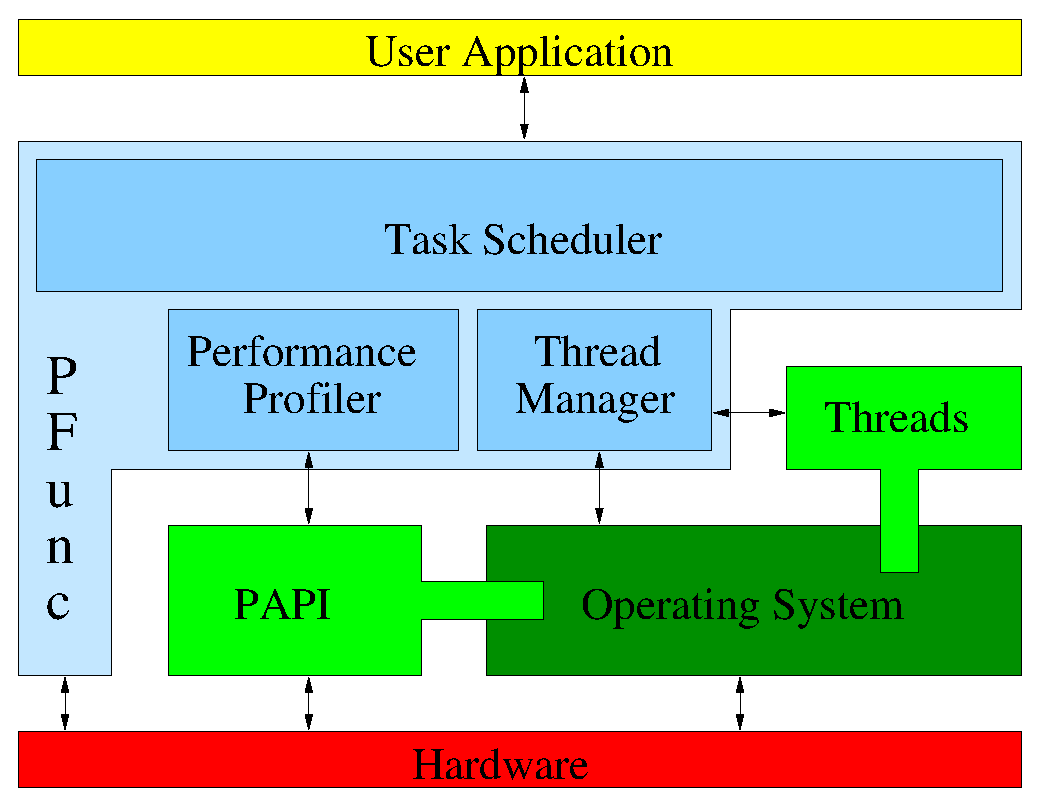
\includegraphics[width=.8\textwidth]{figs/architecture}
\caption{An overview of the software architecture of PFunc; only the relevant
components are shown. Components linked by arrows interface with each other.
Protrusion of one component into another implies that a part of the former
component is implemented in the latter (e.g., threads are partly implemented in
the operating system). Performance Application Profiling Interface (PAPI) is a
profiling library used for collecting hardware statistics.}
\label{fig:software_architecture}
\end{figure}

\subsection{Components of PFunc}
\label{subsec:pfunc_components}

The design of PFunc revolves around providing users control over six ``little
details'' related to task execution: priorities, scheduling, stealing,
affinities, graph structure, and groups.
%
As PFunc's design is ``lifted'' from the designs of existing task parallel
solutions, many components in PFunc correspond one-to-one with components in
other task parallel solutions with one important difference --- PFunc's
components can be configured and/or extended.
%
As shown in Figure~\ref{fig:runtime}, PFunc's components fit into three
categories: \textit{user-provided} (gold colored), \textit{generated} (pink
colored), and \textit{fixed} (blue colored).
%
User-provided components (work, task queue, and task predicates) are
implemented by the users to suit their needs.  
%
The task queue and the task predicate components from a logical grouping called
the task scheduler.
%
PFunc provides a number of built-in choices for the user-provided components;
hence, for many applications, PFunc works ``out-of-the-box''. 
%
However, if these built-in choices do not meet the users requirements, they may 
implement their own user-provided components.
%
Generated components (attribute, task, and task manager) are automatically
created at compile-time using information from the user-provided components.
%
The user-provided and generated components can be configured and/or extended to
create a variety of configurations of PFunc (see Section~\ref{sec:custom}).
%
Fixed components are non-configurable and include group, thread manager,
exception handler, and performance profiler.
%
In practice, PFunc components are implemented as \Cpp{} classes; hence, PFunc
at runtime consists of one or more objects of these classes that are
interacting with each other.
%

\begin{figure}
\centering
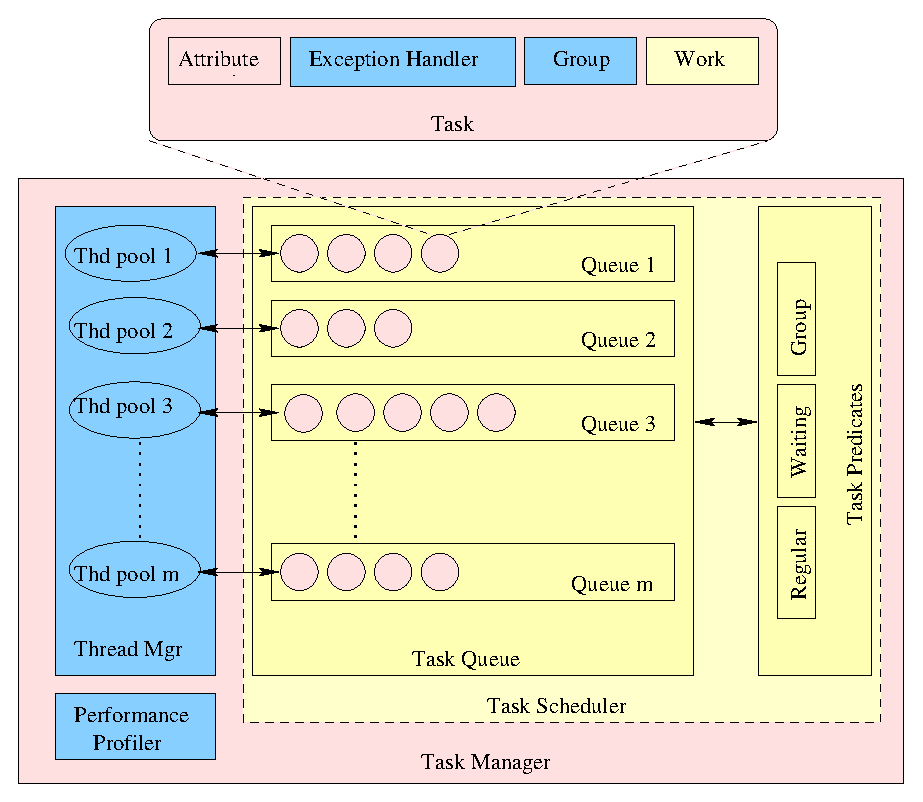
\includegraphics[width=0.8\textwidth]{figs/runtime}
\caption{An overview of the different components in PFunc at runtime.
Components colored yellow (task queue, task predicate, and work) are
user-provided. Components colored pink (attribute, task, and task manager) are
generated. Components colored blue are fixed. PFunc allows users to customize
both the user-provided and generated components.}
\label{fig:runtime}
\end{figure}

\subsection{User-provided Components}
\label{subsec:user_provided}

\subsubsection{Task Scheduler}
%
This component is a logical grouping of the task queue and the task predicate
components.
%
The task scheduler is primarily responsible for choosing the next task to be
executed by each thread. 
%
The task queue and the task predicate components are chosen at compile-time
based on the task scheduling policy selected by the user (see
Section~\ref{sec:custom}).
%
Users can choose from one of the four built-in scheduling policies
(\code{cilkS}, \code{prioS}, \code{lifoS}, and \code{fifoS}) or choose to 
implement their own scheduling policy.
%
For the built-in scheduling policies, the task queue and task predicate
components are pre-defined.
%
However, if users choose to implement their own scheduling policy, they must 
define the task queue and the task predicate components.
%
 
There are two situations in which the task scheduler is used: when a task
is spawned and inserted into a task queue, and when a thread is ready to
execute a task and this task must be selected from the task queue.
%
There are three scenarios in which a thread is ready to execute a task. 
%
In the first scenario, the thread is idle and is looking for a task to execute; 
this is called a \emph{regular} scheduling point.
%
In the second scenario, the thread suspends the parent task it is executing
because the parent task starts waiting on one or more of its children to
complete execution.  
%
Therefore, a new task must be chosen for this thread to execute; this is called
a \emph{waiting} scheduling point.
%
In the third scenario, the thread suspends execution of a task because the task
has entered a wait for a group barrier operation; this is called a \emph{group}
scheduling point.
%

\paragraph{Task Queue}
%
The task queue manages multiple internal queues that store references to
spawned tasks, and supports two atomic operations: \func{put} and \func{get}.
%
The \func{put} function is used to add a newly spawned task to a user-specified
queue.
%
The \func{get} function is used to retrieve a task from the task queue. 
%
The exact queue from which \func{get} retrieves the task is determined jointly
with the task predicate component. 
%
The nature of the internal queues used by the task queue component reflects the
scheduling policy being implemented.
%
For example, for the \code{cilkS} scheduling policy, \code{std::deque} is used
as the type of each internal queue.
%
Similarly, for the \code{lifoS} scheduling policy, \code{std::stack} is used
as the type of each internal queue.

\paragraph{Task Predicate}
%
This component is composed of three predicate pairs --- one pair of predicates
for each scheduling point. 
%
The \code{regular\_predicate\_pair} is used during the regular scheduling
point, \code{waiting\_predicate\_pair} during the waiting scheduling point, and
\code{group\_predicate\_pair} during the group scheduling point.
%
The first predicate of each pair is used to enforce scheduling when the calling
thread's \emph{own} queue is non-empty; the second predicate of each pair is
used when the calling thread's own queue is empty and a task must be
\emph{stolen} from another queue.
 
%
In conjunction with the task queue, the task predicate helps implement a
variety of scheduling policies.
%
The task predicate is used when a new task has be chosen for execution --- when
any of the three scheduling points  is reached.
%
When a thread needs a task to execute, it (via the task manager) calls the
\func{get} function of the task queue; the predicate pair corresponding to the
scheduling point is determined and passed in as an argument to \func{get}.
%
Then, \func{get} checks if the calling thread's own queue is non-empty. 
%
If it is non-empty, depending on the scheduling policy, candidate tasks are 
selected and the \emph{own} predicate is applied to those tasks.
%
The first candidate task from the calling thread's own queue to satisfy the 
predicate is returned to the calling thread for execution.
%
If the calling thread's own queue is empty or if there are no eligible tasks in
it, \func{get} tries to steal a task from another randomly selected queue, at
which point, the \emph{steal} predicate is used.

\begin{figure}
\centering
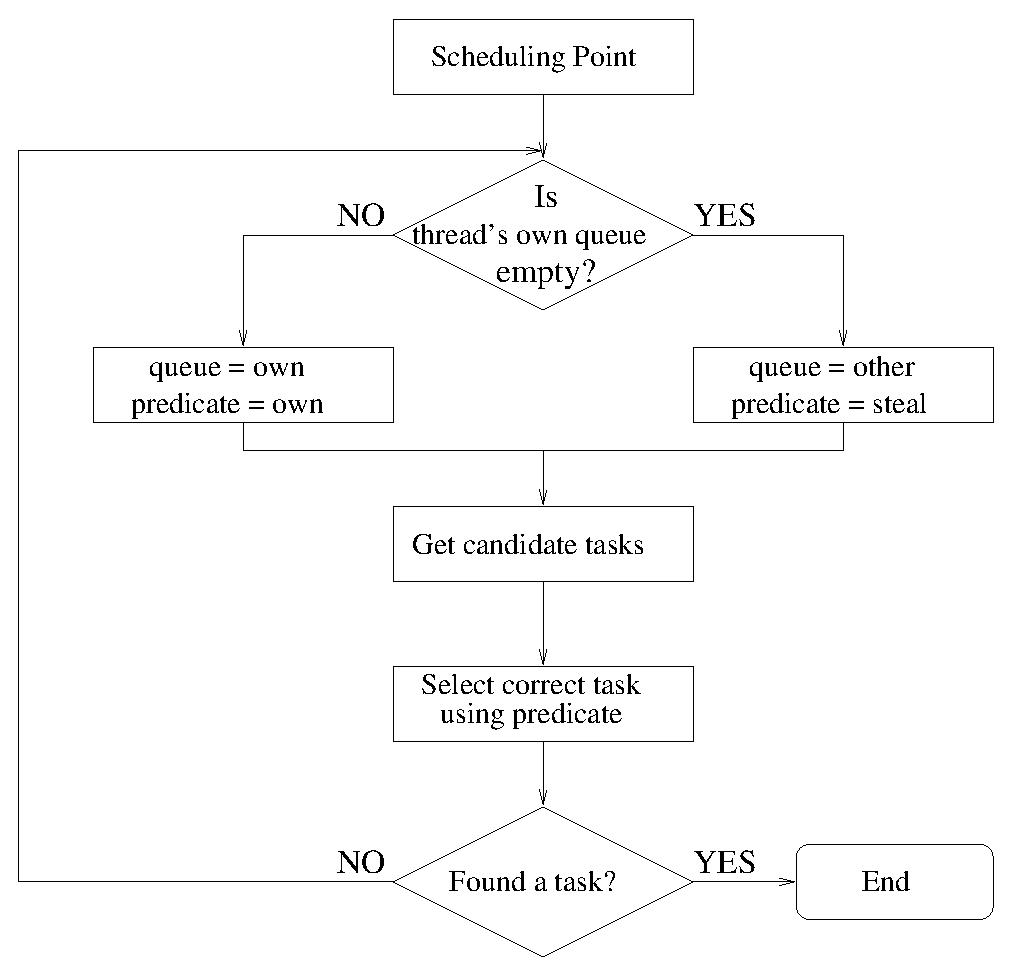
\includegraphics[width=0.7\textwidth]{figs/scheduling}
\caption{Flowchart depicting the task selection process at a scheduling point.}
\label{fig:scheduling}
\end{figure}

\paragraph{Work}
%
The main purpose of PFunc is to enable asynchronous execution of computations.
%
Work is the generic representation of a computation and is a part of the task.
%
In PFunc, computations are restricted to be functions or function objects that 
meet certain constraints.

\subsection{Generated Components}
\label{sec:auto_generated}

\subsubsection{Attribute}
\label{subsubsec:attribute}
%
The attribute component is central in providing users control over ``little
details'' such as scheduling, priority, affinity, task graph structure, and
grouping.
%
Each task contains an attribute, which in turn is made up of six
sub-attributes: \emph{priority}, \emph{queue\_number}, \emph{num\_waiters},
\emph{grouped}, \emph{level}, and \emph{nested}.
%
As there is a task associated with each asynchronous computation, there is also
an attribute associated with each asynchronous computation.
%
To control the execution of a task, users can specify the value for the
required sub-attributes of the task's attribute at the time of spawning.
%
The role of each of these six sub-attributes is summarized below.

\paragraph{priority} Many task scheduling policies require that tasks 
themselves provide hints to help scheduling.
%
For example, the built-in \code{prioS} scheduling policy requires each task to
have a priority.
%
The priority sub-attribute can be used to provide hints to the scheduler
component to help realize customized scheduling policies.
 
\paragraph{queue\_number} PFunc allows control over the affinity of a task
by allowing users to specify the task queue (numbered $[0..n)$, where $n$ is 
the total number of queues) on which the task must be spawned.
%
This is a departure from the methodology of existing solutions for task
parallelism, where a task is always put on the queue serviced by the spawning
thread. 
%
In PFunc, the task is put on the queue serviced by the spawning thread only
if a queue number is not specified while spawning the task.
 
\paragraph{num\_waiters} In PFunc, a task can have multiple parents, which 
results in the task graph structure being a DAG, not just a tree.
%
To support DAG-shaped task graph structures, it is necessary to be able to 
deliver status notifications regarding a task to all its parents.
%
The value of the num\_waiters sub-attribute gives the number of parents for the
task.
%
If this sub-attribute is unspecified for a task, that particular task is
assumed to have a single parent.
 
\paragraph{grouped} PFunc supports SPMD-style parallelization through task
groups.
%
When a task is part of a group, it is automatically given a \emph{rank} in the 
group, which it can use to communicate with the members of its own group.
%
However, when a task is attached to a group, extra instructions are added to 
the critical path (see Section~\ref{subsubsec:group}); therefore, tasks that
use PFunc's group infrastructure incur a performance penalty.
%
To avoid performance loss incurred from a task's membership in a group, the
grouped sub-attribute can be modified so that PFunc only associates the task
with its group when necessary.
%
Most task parallel programs do not make use of groups; by default, tasks are
not attached to \textit{any} group (i.e., grouped sub-attribute is unset)

\paragraph{level} This sub-attribute is used by the task scheduler to
ensure that the thread does not exhaust its stack space by stealing
incorrectly.
%
An important function of the task scheduler component is to ensure that the
underlying system resources are not exhausted. 
%
Thread stack space is one such resource.
%
In PFunc, three of the built-in scheduling policies (\code{cilkS},
\code{lifoS}, and \code{fifoS}) utilize the level sub-attribute to accurately
determine the depth of a task in the task graph.
%
Then, by enforcing a stealing predicate that prohibits a thread from stealing
tasks that are higher (closer to the root) in the task graph than the task 
currently suspended by the thread, thread stack space is conserved.
%

\paragraph{nested} PFunc inherently supports nested parallelism, in which
a task is allowed to spawn other tasks recursively.
%
As there may be more tasks than threads, to support nested parallelism we
need to suspend a parent task to execute a child task.
%
Such task suspension is automatically carried out at both the waiting and 
group scheduling points.
%
However, PFunc's nested sub-attribute allows users to prevent automatic task
suspension at these synchronization points by turning off nested parallelism at
the task level.
%

\subsubsection{Task}
\label{subsubsec:task}
%
The task is PFunc's representation of an asynchronous computation; it contains
the attribute, group, exception handler, and work that is related to the
computation's execution.
%
There is one ``active'' task for each spawned computation.
%
Task interfaces with users on one end and the task scheduler and task manager
on the other end.
%
When a spawned computation completes its execution, the task delivers its
completion notifications to all its parent tasks.
%
The number of completion notifications delivered depends on that particular
task's num\_parents sub-attribute.
%
After all the completion notifications have been delivered, the task is 
terminated; at this point, the task is ``inactive'' and can be used to spawn 
another asynchronous computation.
%
When a task enters either a waiting or group scheduling point, if the task is 
nested, the task triggers the task manager; the task manager in turn starts a
scheduling cycle.
%

\subsubsection{Task Manager}
\label{subsubsec:task_manager}

The task manager is PFunc's runtime; it is the component that glues together
the task, task scheduler, thread manager, and performance profiler components.
%
The task manager's responsibilities can be fit into three categories:
initialization, scheduling, and shut down.
 
\paragraph{Initialization:} During initialization, users provide two pieces of
information: the number of task queues and the number of threads per task
queue.
%
The task manager uses this information to create the specified number of task 
queues and attaches the requested number of threads to each queue. 
%
With this facility, users can create an $m\times{}n$ mapping between queues and
threads.
%
When $m=n$, there is one thread attached to each queue; this is called the 
\emph{work-stealing} configuration.
%
When $m=1$, there is one queue to which all $n$ threads are attached; this is
called the \emph{work-sharing} configuration.
%
Optionally, users can also specify both the affinity of each thread to
individual processors, and the hardware statistics to be collected (see
Section~\ref{sec:perf}).
%
At the end of initialization, the task scheduler, the thread manager, and
the performance profiler are configured, and the task manager is ready to be
used to spawn and execute tasks asynchronously.

\paragraph{Scheduling:} This phase can alternately be called the
\emph{spawn-execute-sync} phase. 
%
When a task is spawned, the task manager is responsible for placing it in the
appropriate queue.
%
When a thread reaches a tasks scheduling point, the thread manager interfaces
with the task scheduler to retrieve an eligible task for this thread to
execute.
%

\paragraph{Shut down:} When the library runtime is no longer needed,
the task manager is responsible for the cleanup of system resources.

\subsection{Fixed Components}
\label{subsec:fixed}

\subsubsection{Group}
\label{subsubsec:group}
%
It is difficult to express all segments of a program in the task parallel
model, therefore, PFunc allows users to mix task parallelism with SPMD-style
programming.
%
The group component is central in providing the support required for SPMD-style
programming. 
%
A task is allowed to be a member of only one group, and group membership is
assigned to a task at the time of spawning.
%
Tasks within the same group can communicate using built-in synchronization
operations. 
%
Each group has the following three pieces of information associated with it:

% Id
\paragraph{Id} This is an integer that uniquely identifies each group and
may be used for debugging purposes.
% Size
\paragraph{Size} Also an integer, this specifies the maximum number of
tasks allowed in the group.
%
The group component can be enabled or disabled for each individual task at
spawn time using the grouped sub-attribute (see
Section~\ref{subsubsec:attribute}).
%
When a task is spawned with its grouped sub-attribute enabled, that task is
given a unique rank in the group at the time of spawning.
%
The rank of a task is an integer in the range $[0..Size)$, and is valid only
when the task is ``active''.
% Barrier
\paragraph{Barrier type} PFunc provides three types of barriers:
\emph{spinning}, \emph{waiting}, and \emph{stealing}. 
%
The value of the barrier type determines which of the three barriers is in use.
%
Spinning barriers are the default.
%
Threads executing tasks in a spinning barrier are incapable of executing other
tasks while these tasks wait on the barrier because the threads must actively
poll for barrier completion.
%
Consequently, the spinning barrier is most useful when all the tasks involved
in the barrier are tightly coupled.
%
Furthermore, for the spinning barrier to work properly, there must be a 
separate thread for each task executing the barrier.
% 
In other words, the size of the group must be less than or equal to the number
of threads used to execute the library instance, or a deadlock may occur.
%
Waiting barriers are useful when system resources need to be conserved. 
%
In waiting barriers, the thread executing a blocked task is suspended from
execution until the barrier is completed.
%
Like the spinning barrier, the waiting barrier also requires that the size of
the group be less than or equal to the number of threads in the system.
%
Finally, stealing barriers offer the speed of spinning barriers and the
efficiency of waiting barriers.
%
When a task is waiting at a stealing barrier, the thread that is executing the
task can suspend the task and execute another eligible task.
%
Therefore, if the tasks involved in a barrier are not tightly coupled, the 
threads executing these tasks can do useful work.
%
The stealing barrier also requires that the number of tasks in the group be
less than or equal to the number of threads.
%
This constraint is a result of the lack of support for true task suspension in
PFunc.\footnote{True task suspension requires that the entire task (with its
stack) be suspended and later resumed by any other thread}. 
%

\subsubsection{Thread Manager}
\label{subsubsec:thread_manager}
%
As PFunc operates exclusively in shared memory, it makes uses of system threads
to execute its tasks.
%
This component is an abstraction that provides portable means of launching,
killing, and yielding threads on various platforms.
%
When PFunc is initialized, the thread manager launches as many threads as
requested and makes them available to service specific task queues.
%
Also, when the underlying system allows for it, the thread manager provides a
portable means of setting each thread's processor affinities --- an important
requirement for optimal performance of many applications.
%
This feature can be used in conjunction with the task attribute to control the
physical processors on which individual tasks are executed.
%
For example, during library initialization, users can tie individual threads 
down to particular processors and determine the task queues serviced by these
threads.
%
Then, using the affinity sub-attribute, tasks can be spawned on particular queues.

\subsubsection{Exception Handler}
\label{subsubsec:exception_handler}

The exception handler aids users in the development of robust applications by
ensuring sensible handling of exceptions in a parallel environment.
%
A parallel execution environment presents two challenges with respect to
exception handling. 
%
First, many PFunc routines are inserted between the child (callee) task which
is throwing the exception and the parent (caller) task that is catching it. 
%
Furthermore, the child and the parent tasks may be executed by different
threads. 
%
Therefore, exceptions need to be transported across many functions and/or
threads.
%
Second, unlike in a sequential environment, the parent task's execution is not always 
suspended until its child task returns. 
%
Therefore, an exception thrown by a task must be stored safely until its parent
task is ready to handle the exception (i.e., waits for the completion of the
throwing task).
%
PFunc's exception handler not only tackles both these challenges, but is also 
capable of delivering exception objects to multiple parent tasks.
%
Therefore, users can handle exceptions as if they were running a sequential
program. 
%
                                
The exception handler defines a new exception class, \code{pfunc::exception},
which extends \code{std::exception} to provide two additional pieces of
information to the users. 
%
First, the trace of the tasks and/or functions through which an exception
object was transported is exposed to the users.
%
Second, if a task terminated as a result of a failed system call or an error
internal to PFunc, this error code is provided to the users.
%
When a task throws an exception, the task is terminated (deactivated) and the
thrown exception is cloned and stored within the task (which is inactive).
%
Cloning is necessary in order to transport the exceptions across multiple tasks
and/or functions without loss of information.
%
Cloning requires that the exceptions objects inherit from either
\code{pfunc::exception} or \code{std::exception}; exception objects that do not
meet this requirement are discarded and a \code{pfunc::exception} with an
``unknown error'' description is propagated in their place.
%
As exception objects may need to be transported from a deeply-nested task to a
top-level task, \code{pfunc::exception} also allows users to add tracing
information that can be used to like a pseudo stack trace.
%
After additional tracing information has been added, the exception object can
be re-thrown to the next higher-level task.
% 

Unfortunately, the exception handler has two shortcomings. 
%
First, when a parent task waits on its children to complete, the exception 
handler must actively check for exceptions.
%
This adds an extra branch in the critical path and results in a small
performance penalty.
%
To remedy this, the exception handler component is disabled by default, and 
can be enabled using a compile-time flag.
%
Second, when a task throws an exception, all the tasks spawned by the throwing
task may have to be cancelled --- a capability that is currently
lacking in the exception handler.

\subsubsection{Performance Profiler}
\label{subsubsec:performance_profiler}

Achieving optimal parallel performance often requires tuning various parameters
such as task scheduling policy, task affinities, etc.
%
To help with such tuning, PFunc provides a performance profiler component that
allows users to collect various hardware statistics related to their
application run.
%
To collect the hardware statistics, this component interfaces with the
Performance Application Programming Interface (PAPI), a production-grade,
open-source, and portable low-level interface.
%
The performance profiler component allows users to specify particular events
(both PAPI presets and native) that they wish to monitor at the time of library
initialization.
%
Then, using PAPI, the performance profiler collects the required hardware 
statistics that can be retrieved at the end of the application run.
%
Shortly, the performance profiler will also be able to collect various
statistics about PFunc's components (e.g., number of steals per thread and load
per thread) that occurred during an application run.
%


\pagebreak

\section{Customizing PFunc} 
\label{sec:custom}

The novelty of PFunc is that many of its runtime components can be configured
and/or extended using generic programming techniques.
%
PFunc's policy-based design allows users to customize its
user-provided components, and indirectly, the generated components as well
through three key features: \emph{scheduling policy}, \emph{compare}, and
\emph{work}.
%
These features directly influence the selection and composition of the
different components that are used in PFunc at runtime.
%
Furthermore, underlying the features are different concepts, which the values
chosen for these features must model.
%
Figure~\ref{fig:custom} depicts the role played by each feature in the
selection of the different components of PFunc.
%
To assist application parallelization ``out-of-the-box'', PFunc provides a 
number of built-in choices for each feature.
%
In this section, we explore the scheduling policy, compare, and work features,
their related concepts, and their built-in values in detail.

There are many different ways of representing concepts and their models.
%
In this section, all the concepts and their models are defined using the syntax
of \ConceptCpp{}, a proposal to add direct support for concepts into the \Cpp{}
language.
%
An important reason for choosing \ConceptCpp{} is that we are able to test the
correctness of our concepts and their models using the reference ConceptGCC
compiler implementation.\footnote{ConceptGCC does not handle templated
associated functions; such functions had to be commented out.}
%
For the sake of brevity, the concepts defined in PFunc make use of other
\emph{external concepts}; these are summarized in
Table~\ref{tbl:external_concepts}.
%
As can be seen, PFunc makes use of concepts from two sources: the \ConceptCpp{}
proposal and the Silicon Graphics International's (SGI) version of the STL.

\begin{figure}
\centering
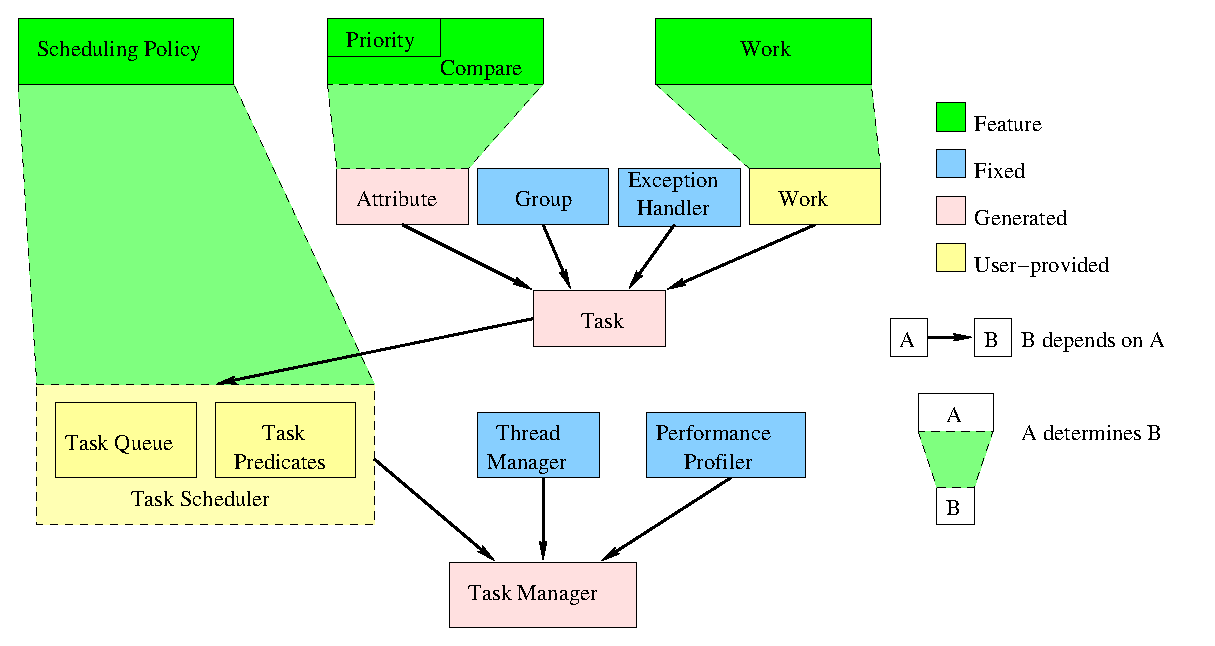
\includegraphics[width=1.0\textwidth]{figs/custom}
\caption{An overview of the configuration diagram for PFunc. PFunc provides
three features (colored green; scheduling policy, compare, and work) that can
be used to generate a variety of library instance descriptions.  Components
colored yellow are user-provided and are either selected from a built-in list
or are implemented by users. Components colored pink are generated from values
given to the three features. Components colored blue are fixed, and hence, are 
not configurable at compile time.}
\label{fig:custom}
\end{figure}

\begin{table}[t]
\centering
\tablefont
\begin{tabular}{|c|c|l|}
\hline
Concept name & Parameters & Description \\
\hline
\concept{Copy Constructible} & \code{T} & Requires the ability to create and destroy copies of objects of type \code{T}. \\
\hline
\concept{Copy Assignable} & \code{T} & Requires the ability to assign values to objects of type \code{T}. \\
\hline
\concept{Default Constructible} & \code{T} & Requires the existence of an accessible default constructor for type \code{T}.\\
\hline
\concept{Same Type} & \code{T1}, \code{T2} & Requires that both \code{T1} and \code{T2} have the exact same type. \\
\hline
\concept{CallableN} & \code{F}, \code{T1}, ..., \code{TN} & Represents a family of concepts (\concept{Callable0}, \concept{Callable1}, ..., \concept{CallableN}). \\
                    & & Requires that \code{F} be callable with given arguments of type \code{T1}, \code{T2}, ... \code{TN}. \\
                    & & Requires that \code{result\_type} be a nested type. \\
\hline
\concept{Adaptable Binary Function} & \code{F}, \code{T1}, \code{T2} & Requires that \code{F} be callable with arguments of type \code{T1} and {T2}. \\
                          & & Requires that \code{first\_argument\_type} and \code{second\_argument\_type} be nested types. \\
                          & & Requires that \code{result\_type} be a nested type. \\
\hline
\end{tabular}
\caption{A summary of all the external concepts that are used in PFunc. All the
listed concepts (other than the \concept{Adaptable Binary Function} concept)
are defined in \ConceptCpp{}. The \concept{Binary Function} concept is
defined in the Silicon Graphics International's (SGI) STL technical
archives.}
\label{tbl:external_concepts}
\end{table}

\subsection{Generator}
\label{subsec:lib_instance}

Like the STL, PFunc is a library template ; in order to use it, users are first
required to generate a concrete library instance description by providing
appropriate values to the three customizable features.
%
These features not only represent the values for the user-provided components,
but also are used to create concrete instances of the generated components. 
%
To facilitate this process, PFunc provides \code{pfunc::generator}, a templated
generator class that accepts three template parameters, each of which represent
a value of a particular feature.
%
The definition of \code{pfunc::generator} is given below:

\begin{lstlisting}[columns=flexible]
template <typename PolicyName, typename Compare, typename Work>
  requires SchedulingPolicy<PolicyName, pfunc::detail::task<Compare, Work> > &&
           AdaptableCallableN<Compare> &&
           Callable0<Work>
struct pfunc::generator { 
  /* type definitions for user-provided and generated components */ 
};
\end{lstlisting}
 
As can be seen, each template parameter (feature) is constrained with
corresponding concept requirements.
%
First, \code{PolicyName} must be a model of the \concept{Scheduling Policy}
concept, defined in Section~\ref{subsec:scheduling_policy}.
%
This concept takes in an additional parameter, \code{TaskType} (represented 
by the template type \code{pfunc::detail::task<T,U>}) that must be a model of
the \concept{PFunc Task} concept defined in
Figure~\ref{fig:pfunc_task_concept}.
%
Second, \code{Compare} is constrained to be a model of one of the the
\concept{Adaptable CallableN} family of concepts, defined in
Section~\ref{subsec:compare}.
%
Finally, \code{Work} must be a model of the \concept{Callable0} concept,
defined in \ConceptCpp{}.

To make PFunc work ``out-of-the-box'', we provide \code{pfunc::use\_default}, a
special class that can be used as the default value of any feature.
%
Specialization of \code{pfunc::generator} for different positional combinations
of \code{pfunc::use\_default} is used to substitute appropriate built-in values
as defaults for each feature (\code{cilkS} for \code{PolicyName},
\code{std::less<int>} for \code{Compare}, and
\code{pfunc::detail::virtual\_functor} for \code{Work}).
%
Once the three template parameters are specified, the library instance
description is generated; this instance exposes the required PFunc components
(work, attribute, group, task, and task manager) as nested types, which are
required to parallelize user applications.

\subsection{Scheduling Policy}
\label{subsec:scheduling_policy}

The value given to this feature determines the scheduling policy that is
used in the generated library instance description; that is, it determines the
task queue and task predicate components.
%
PFunc offers four built-in values for this feature: \code{cilkS}, \code{prioS},
\code{lifoS}, and \code{fifoS}; in addition, users can define custom scheduling
polices.
%
Values given to the scheduling policy feature must model the
\concept{Scheduling Policy} concept, defined below.
%
\begin{lstlisting}
concept SchedulingPolicy <typename PolicyName, typename TaskType> {
  /* concept requirements */
  requires PFuncTask <TaskType>;
  @\halfline@
  /* associated types */
  typename task_queue_set;
  typename regular_predicate_pair;
  typename waiting_predicate_pair;
  typename group_predicate_pair;
  @\halfline@
  /* associated type requirements */
  requires TaskQueueSet <PolicyName, task_queue_set>;
  requires TaskPredicatePair <PolicyName, regular_predicate_pair>;
  requires SameType <TaskType*, regular_predicate_pair::value_type>;
  requires TaskPredicatePair <PolicyName, waiting_predicate_pair>;
  requires SameType <TaskType*, waiting_predicate_pair::value_type>;
  requires TaskPredicatePair <PolicyName, group_predicate_pair>;
  requires SameType <TaskType*, group_predicate_pair::value_type>;
}
\end{lstlisting}
%
The \concept{Scheduling Policy} concept takes two parameters: \code{PolicyName}
and \code{TaskType}.
%
\code{TaskType}, the second (additional) parameter, is required because it
influences the type of the components (task queue and task predicate) that
implement the scheduling policy.
%
Any type used as \code{TaskType} is required to model the \concept{PFunc Task}
concept defined in Figure~\ref{fig:pfunc_task_concept}.
%
In PFunc, the task is a generated component whose type is jointly determined by
the values of both the compare and work features; it is represented by the
template type \code{pfunc::detail::task<T,U>}.
%
Briefly, the \concept{PFunc Task} concept stipulates that any valid
\code{TaskType} must be a model of both \concept{Copy Constructible} and
\concept{Copy Assignable} concepts.
%
Furthermore, it is required to have \code{compare\_type} and \code{work\_type}
as associated types.
%
In turn, \code{compare\_type} is required to be a model of one of the concepts
in the \concept{Adaptable CallableN} family of concepts (see
Section~\ref{subsec:compare}) and \code{work\_type} is required to be a model
of the \concept{Callable0} concept (see Section~\ref{subsec:custom_work}).
%
Finally, \code{TaskType} must define the \func{TaskType::get\_compare}
associated function, which returns returns an object of type
\code{compare\_type} when it is invoked.
%
\begin{figure}
\begin{center}
\begin{minipage}{0.8\textwidth}
\begin{lstlisting}[frame=trbl]
concept PFuncTask <typename TaskType> {
  /* concept requirements */
  requires CopyConstructible <TaskType> && CopyAssignable <TaskType>;
  @\halfline@
  /* associated types */
  typename compare_type;
  typename work_type;
  @\halfline@
  /* associated type requirements */
  requires AdaptableCallableN<compare_type>;
  requires Callable0<work_type>;
  @\halfline@
  /* associate functions */
  compare_type TaskType::get_compare () const;
}
\end{lstlisting}
\end{minipage}
\end{center}
\caption{The concept definition of the \concept{PFunc Task} concept, which
governs type of the task objects in PFunc (of type \code{TaskType}.)}
\label{fig:pfunc_task_concept}
\end{figure}
%
Models of the \concept{Scheduling Policy} concept must define four
associated types: \code{task\_queue\_set}, \code{regular\_predicate\_pair},
\code{waiting\_predicate\_pair}, and \code{group\_predicate\_pair}.
%
Of these, the \code{task\_queue\_set} associated type represents the task queue
component and must be a model of the \concept{Task Queue Set} concept (defined
in Section~\ref{subsubsec:task_queue_set}).
%
The remaining three associated types together form the task predicate component
and must be models of the \concept{Task Predicate Pair} concept, which is
defined in Section~\ref{subsubsec:task_predicate}.

\subsubsection{Task Predicate Pair}
\label{subsubsec:task_predicate}
%
Every scheduling policy must define the three predicate pairs that form the
task predicate component; each pair must model the \concept{Task Predicate
Pair} concept, defined below.

\begin{lstlisting}
concept TaskPredicatePair <typename PolicyName, typename PredPair> {
  /* associated types */
  typename value_type;
  typename result_type;
  @\halfline@
  /* associated functions */
  PredPair::PredPair(value_type);
  result_type PredPair::own_pred(value_type);
  result_type PredPair::steal_pred(value_type);
}
\end{lstlisting}
% 
The \concept{Task Predicate Pair} concept takes two parameters:
\code{PolicyName} and \code{PredPair}. 
%
In other words, \concept{Task Predicate Pair} ensures that \code{PredPair} can
be used by the scheduling policy defined by \code{PolicyName}.
%
The \concept{Task Predicate Pair} concept defines two associated types: 
\code{value\_type} and \code{result\_type}, and three associated functions:
\func{PredPair::PredPair}, \func{own\_pred}, and \func{steal\_pred}.
%
Like the \code{PolicyName}, the \code{value\_type} associated type is used to 
ensure compatibility between the task predicate and task scheduling components.
%
At each scheduling point, the thread manager constructs a new \code{PredPair}
corresponding to the type of the scheduling point, and passes it as an argument
to the task queue component.
%
Therefore, the time required to construct a predicate pair directly adds to
the task scheduling overhead, and it is advisable to have \emph{light} task
predicates that can be constructed quickly.
%
New predicate pairs are constructed by invoking their respective initializing
constructors (\func{PredPair::PredPair}); at this time, these predicates are
passed a pointer to the task previously executed by the calling thread.
%
This (task) pointer contains information about the previously executed task's
attributes, which can be used by the task queue component to evaluate the
goodness of the candidate tasks when picking the next task to execute.
%
To evaluate the candidate tasks in the calling thread's own queue, the
\func{PredPair::own\_pred} associated function is used; else (when stealing),
the \func{PredPair::steal\_pred} associated function is used.

\subsubsection{Task Queue Set}
\label{subsubsec:task_queue_set}
%
For a policy to be a valid value of the scheduling policy feature, it must
define a task queue component. 
%
The task queue component is governed by the \concept{Task Queue Set} concept
defined below.

\begin{lstlisting}[columns=flexible]
concept TaskQueueSet <typename PolicyName, typename QueueSet> {
  /* associated types */
  typename value_type;
  typename queue_index_type;
  @\halfline@
  /* associated type requirements */
  requires PFuncTask <remove_pointer<value_type>::result_type>;
  requires CopyConstructible <queue_index_type> && 
           CopyAssignable <queue_index_type> &&
           DefaultConstructible <queue_index_type>;
  @\halfline@
  /* associated functions */
  QueueSet::QueueSet (unsigned int);
  void QueueSet::put (queue_index_type, const value_type&);
  template <typename PredPair>
  requires TaskPredicatePair<PredPair, PolicyName> &&
           SameType<TaskPredicatePair<PredPair, PolicyName>::value_type, value_type>
  value_type QueueSet::get (queue_index_type, const PredPair&);
};
\end{lstlisting}

The \concept{Task Queue Set} concept takes two parameters: \code{PolicyName}
and \code{QueueSet}.
%
In other words, \concept{Task Queue Set} ensures that \code{QueueSet} can
be used by the scheduling policy defined by \code{PolicyName}.
%
Models of the \concept{Task Queue Set} concept manage one or more internal
queues, which contain elements of type \code{value\_type}, which is
\textit{always} a pointer to the instantiated task type; PFunc's task type's
requirements are captured by the \concept{PFunc Task} described in
Figure~\ref{fig:pfunc_task_concept}.
%
Users can spawn tasks on an individual (internal) queue by specifying the
queue's index in objects of type \code{QueueSet}.
%
Queue indices are of the type \code{queue\_index\_type}; this type is required
to be a model of the \concept{Copy Constructible}, \concept{Copy Assignable},
and \concept{Default Constructible} concepts.
%
\concept{Task Queue Set} provides three associated functions:
\func{QueueSet::QueueSet} to construct a new queue set with the required number
of queues, and \func{QueueSet::put} and \func{QueueSet::get}, which allow
atomic insertion and removal of elements from the selected internal queue.
%
The second argument to \func{QueueSet::get} is a predicate pair that is
required to be a model of the \concept{Task Predicate Pair} concept (for the
same \code{PolicyName}).
%
In addition, the \code{value\_type} associated type of both \code{QueueSet}
and \code{PredPair} are required to be of the same type (enforced by the
\concept{Same Type} concept).
%

\subsubsection{Example}
\label{subsubsec:scheduling_example}
%
We illustrate the process of implementing a custom scheduling policy using the
built-in \code{fifoS} policy as an example. 
%
Notice that in practice, as concepts are not yet supported by the existing 
\Cpp{} standards, we realize concepts mostly through specialization and 
documentation.
%
First, we define \code{fifoS} as a concrete type so that it can be used as the
\code{PolicyName} to specialize the classes that implement the task queue and
task predicate components.
%

\begin{lstlisting}
struct fifoS {}; 
\end{lstlisting}

\noindent
Next, we need to create the three predicate pairs that are required to
implement the task predicate component for \code{fifoS} scheduling policy.
%
However, PFunc's default implementation of the three predicate pairs suffices
for \code{fifoS}; therefore, we do not need to specialize.
%
For example, consider the default implementation of the
\code{regular_predicate_pair}:
%
\begin{lstlisting}
template <typename PolicyName, typename ValueType>
struct regular_predicate_pair {
  typedef bool result_type;
  typedef ValueType* value_type;
  @\halfline@
  regular_predicate_pair (value_type previous_task=NULL) {}
  @\halfline@
  bool own_pred (value_type current_task) const { return true; }
  @\halfline@
  bool steal_pred (value_type current_task) const { return own_pred (current_task); }
};
\end{lstlisting}
%
\noindent
This default implementation tells the scheduler that there are no additional
stipulations on tasks that are picked from the task queues as both
\func{own_pred} and \func{steal_pred} always return \code{true}.
%
Next, we specialize \code{task_queue_set}, a templatized structure that all 
scheduling policies are required to specialize.
%
\begin{lstlisting}[columns=flexible]
template <typename ValueType>
struct task_queue_set <fifoS, ValueType> {
  typedef std::queue<ValueType*> queue_type;
  typedef typename queue_type::value_type value_type;
  typedef unsigned int queue_index_type; 
  @\halfline@
  task_queue_set (unsigned int num_queues) { /* create num_queue std::queues */ }
  @\halfline@
  template <typename TaskPredicatePair>
  value_type get (queue_index_type queue_num, const TaskPredicatePair& cnd) {
    /* retrieve a task from the set of queues. first, attempt to retrieve from queue_num, then steal */
  }
  @\halfline@
  void put (queue_index_type queue_num, const value_type& value) { 
    /* store at the back of the requested queue */ 
  }
};
\end{lstlisting}
%
\noindent
With the completion of this step, the \code{fifoS} scheduling policy meets all
the requirements of the \concept{Scheduling Policy} concept.
%
Therefore, \code{fifoS} models the \concept{Scheduling Policy} concept and can
be used as a value of the scheduling policy feature.
%
For the complete implementation, please see \code{pfunc/fifo.cpp}.

\subsection{Compare}
\label{subsec:compare}

This feature is used to compare task priorities when the chosen scheduling
policy uses priorities.  
%
PFunc stipulates that the value given to the compare feature should model one
of the concepts in the \concept{Adaptable CallableN} family of concepts; the 
definition of this family of concepts is given below:

\begin{lstlisting}[columns=flexible]
concept AdaptableCallableN <typename Functor> {
  /* concept requirements */
  requires CopyConstructible <Functor> && DefaultConstructible <Functor> && CopyAssignable <Functor>;
  @\halfline@
  /* associated types */
  typename first_argument_type;
  typename result_type;
  @\halfline@
  /* associated type requirements */
  requires CopyConstructible <first_argument_type> && DefaultConstructible <first_argument_type> && 
           CopyAssignable <first_argument_type>;
  requires CallableN <Functor, first_argument_type, ...,first_argument_type>;
  requires SameType <CallableN <Functor, first_argument_type, ...,first_argument_type>::result_type, 
                      result_type>;
}
\end{lstlisting}

The \concept{Adaptable CallableN} family of concepts requires its models to
define two associated types: \code{first\_argument\_type} and
\code{result\_type}.
%
PFunc automatically derives the type of the priority sub-attribute from the
value given to the compare feature; hence, it is necessary to define
\code{first\_argument\_type}.
%
That is, \code{first\_argument\_type} is used as the type of the priority
sub-attribute.
%
Further, a model of one of the concepts in the \concept{Adaptable CallableN}
family of concepts must also model the corresponding concept in the
\concept{CallableN} family of concepts.
%
Furthermore, for a \code{Functor}, \code{result\_type} must be the same in both
the \concept{CallableN} and \concept{Adaptable CallableN} family of concepts;
this constraint is enforced using the \concept{Same Type} concept.
%
For example, a model of the \concept{Adaptable Callable2} concept is required 
to also be a model of the \concept{Callable2} concept, and have the same 
\code{result\_type}.
%
Note that the \concept {Adaptable CallableN} family of concepts inherently
ensures that only a single type can be used as the type of the task priority.
%
Finally, both \code{Functor} and \code{first\_argument\_type} must be a model
of the \concept{Default Constructible}, \concept{Copy Constructible}, and
\concept{Copy Assignable} concepts. 
%
Because the value given to the compare feature influences the type of the
attribute component, it transitively affects the types of the task, task
queue, and task predicate components.

Although PFunc only requires that the value given to the compare feature be a
model of one of the concepts in the \concept{Adaptable CallableN} family of
concepts, a scheduling policy can place additional constraints on the value
given to this feature.
%
For example, the \code{prioS} scheduling policy uses task priorities to enforce
a strict weak ordering; therefore, the value given to the compare feature is
required to be a model of the \concept{Partial Order} concept. 
%
The \concept{Partial Order} concept is a refinement of the \concept{Adaptable
Callable2} concept that requires that its models must be irreflexive,
antisymmetric, and transitive; this concept is defined below.

\begin{lstlisting}[columns=flexible]
concept PartialOrder <typename Functor> : AdaptableCallable2 <Functor> {
  /* concept requirements */
  requires SameType<result_type, bool>;

  axiom Irreflexivity (Functor& f, first_argument_type one) { false == f(one,one); }
  axiom AntiSymmetry (Functor& f, first_argument_type one, first_argument_type two) { 
    if (false==f(one,two)) true == f(two,one);
  }
  axiom Transitivity (Functor& f, first_argument_type one, first_argument_type two, first_argument_type three) {
    if (f(one,two) && f(two,three)) true == f(one,three);
  }
}
\end{lstlisting}

For convenience, PFunc allows programmers to use \code{pfunc::use\_default} as 
the value of the compare feature.
%
This value is then turned into the STL functor \code{std::less<int>}, which 
is a model of the \concept{Partial Order} concept. 
%
In fact, any function object that models the \concept{Adaptable Binary Function} concept
is a model of the \concept{Adaptable Callable2} concept as well (iff the
function parameter types are the same type).

\subsection{Work}
\label{subsec:custom_work}

This feature allows users to specify the type of the function object that is
executed by the tasks.  
%
The value given to this feature must be a model of the \concept{Callable0}
concept.
%
By allowing the type of the function object to be specified as a feature, PFunc
successfully avoids paying the cost of virtual function calls in the spawned
tasks when there is only one type of function object to parallelize.
%
This is unlike other libraries such as TBB, in which spawning a new task always
incurs the cost of a virtual function call.  
%
However, if more than one type of function object needs to be parallelized, the
cost of a virtual function call cannot be avoided.
%
The value given to the work feature is substituted for the type of \emph{work}
in the task component; therefore, the value given to this feature influences
the type of the work component.
%
Transitively, it also determines the types of the task, task queue, and task
predicate components.
%
Function objects that represent spawned computations are maintained within
PFunc as non-constant references; it is illegal to modify or deallocate the
function object before the associated task is finished.
 
When \code{pfunc::use\_default} is specified as the value of the work feature,
PFunc substitutes it with \code{pfunc::virtual\_functor}, an abstract
base class that is a model of the \concept{Callable0} concept.
%
In this case, all function objects that need to be parallelized must inherit
from the type \code{pfunc::virtual\_functor} in order to be executed in
parallel by PFunc.


\end{document}
